

%*** General probabilistic notation ***

\newcommand{\expv}{\mathbf{E}} % EXP. VALUE
\newcommand{\discProbDist}{f} % Discrete prob distribution
\newcommand{\sampleSpace}{S} % Generic sample space
\newcommand{\sigmaAlg}{\mathcal{F}} % Generic sigma-algebra
\newcommand{\probm}{\mathbb{P}} % Generic probability measure, also prob. measure operator
\newcommand{\rvar}{X} % Generic random variable
%\newcommand{\dist}{\mathit{Dist}}

%*** MDP notation ***

\newcommand{\actions}{A} % The set of actions.
\newcommand{\colouring}{c} % the colouring function
\newcommand{\probTranFunc}{\Delta} % Transition function of an MDP
\newcommand{\edges}{E} % Set of edges in an MDP.
\newcommand{\colours}{C} % The set of colours in an MDP.
\newcommand{\mdp}{\mathcal{M}} % A generic MDP. 
\newcommand{\vinit}{v_0} % An initial vertex in an MDP.
\newcommand{\cylProb}{p} % Function assigning probabilities to cylinder sets in 
%the measure construction.
\newcommand{\emptyPlay}{\epsilon} %empty play
\newcommand{\objective}{\Omega} % Qualitative objective
\newcommand{\genColour}{\textsc{c}} % Generic colour
\newcommand{\quantObj}{f} % Generic quantitative objective
\newcommand{\indicator}[1]{\mathbf{1}_{#1}} % In.d RV
\newcommand{\eps}{\varepsilon} % Numerical epsilon
\newcommand{\maxc}{W} % Maximal abs. value of a colour

\newcommand{\winPos}{W_{>0}}
\newcommand{\winAS}{W_{=1}}
\newcommand{\cylinder}{\mathit{Cyl}}

\newcommand{\PrePos}{\text{Pre}_{>0}}
\newcommand{\PreAS}{\text{Pre}_{=1}}

\newcommand{\PreOPPos}{\mathcal{P}_{>0}}
\newcommand{\OPAS}{\mathcal{P}_{=1}}

\newcommand{\safeOP}{\mathit{Safe_{=1}}}
\newcommand{\closed}{\mathit{Cl}}

\newcommand{\reachOP}{\mathcal{V}}
\newcommand{\discOP}{\mathcal{D}}
\newcommand{\valsigma}{\vec{x}^{\sigma}}

\newcommand{\lp}{\mathcal{L}}
\newcommand{\lpdisc}{\lp_{\mathit{disc}}}
\newcommand{\lpmp}{\lp_{\mathit{mp}}}
\newcommand{\lpsol}[1]{\bar{#1}}
\newcommand{\lpmpdual}{\lpmp^{\mathit{dual}}}

\newcommand{\actevent}[3]{\actions^{#1}_{#2,#3}} % Returns #1-th action on the run 

\newcommand{\MeanPayoffSup}{\MeanPayoff^{+}}
\newcommand{\MeanPayoffInf}{\MeanPayoff^{-}}

\newcommand{\mcprob}{M}
\newcommand{\invdist}{\vec{z}}

\newcommand{\hittime}{T}


%\usepackage{xspace}

\newcommand{\Win}{\textsc{Win}\xspace} 
\newcommand{\Lose}{\textsc{Lose}\xspace} 

%%%%%%%%%%%%%%%%%%%%%% Colors
%% all colors
\colorlet{grey-10}{black!10!white}
\colorlet{grey-20}{black!20!white}
\colorlet{grey-30}{black!30!white}
\colorlet{grey-40}{black!40!white}
\colorlet{grey-50}{black!50!white}
\colorlet{grey-60}{black!60!white}

\colorlet{lgrey-back}{black!10!white}
\colorlet{lgrey-border}{black!40!white}
\colorlet{dgrey-back}{black!30!white}
\colorlet{dgrey-border}{black!80!white}

%% default
\colorlet{state-back}{lgrey-back}
\colorlet{state-border}{lgrey-border}

%%%%%%%%%%%%%%%%%%%%%% Tikzstyles
%% background+border
\tikzstyle{grey}=[fill=lgrey-back,draw=lgrey-border]
\tikzstyle{lgrey}=[grey]
\tikzstyle{dgrey}=[fill=dgrey-back,draw=dgrey-border]
\tikzstyle{white}=[fill=white,draw=black]
\tikzstyle{black}=[fill=black,draw=black]

%% states
\tikzstyle{@state}=[fill=state-back,draw=state-border,inner sep=0pt,line width=.8pt]
\tikzstyle{square16}=[@state,rectangle,minimum height=16mm,minimum width=16mm]
\tikzstyle{square10}=[@state,rectangle,minimum height=10mm,minimum width=10mm]
\tikzstyle{square5}=[@state,rectangle,minimum height=5mm,minimum width=5mm]
\tikzstyle{square4}=[@state,rectangle,minimum height=4mm,minimum width=4mm]
\tikzstyle{circle6}=[@state,circle,minimum size=6mm]
\tikzstyle{circle4}=[@state,circle,minimum size=4.3mm]
\tikzstyle{diamond7}=[@state,diamond,minimum height=7.5mm,minimum width=7.5mm]
\tikzstyle{diamond5}=[@state,diamond,minimum height=5mm,minimum width=5mm]
\tikzstyle{state}=[s-eve]
\tikzstyle{s-eve}=[circle6]
\tikzstyle{s-adam}=[square5]
\tikzstyle{s-random}=[diamond7]
\tikzstyle{s-eve-small}=[circle4]
\tikzstyle{s-adam-small}=[square4]
\tikzstyle{s-random-small}=[diamond5]
\tikzset{node distance=2.5cm}
\tikzset{every node/.style={anchor=base}}

%% edges
\tikzset{>=latex,bend angle=20}
\tikzstyle{line}=[line width=.6pt]
\tikzstyle{arrow}=[->,line]
\tikzstyle{dblarrow}=[<->,line]
\tikzstyle{invarrow}=[<-,line]
\tikzstyle{initial}=[invarrow]
\tikzset{selfloop/.style={arrow,out={#1-30},in={#1+30},looseness=6}}
    % we use tikzset here because tikzstyle does not allow arguments
    

%% diagrams
\tikzstyle{fillarea}=[line width=.6pt,line join=round]
% define new hatch pattern
\newlength{\hatchspread}
\newlength{\hatchthickness}
\tikzset{hatchspread/.code={\setlength{\hatchspread}{#1}},
  hatchthickness/.code={\setlength{\hatchthickness}{#1}}}
\tikzset{hatchspread=3pt,hatchthickness=0.4pt}
\pgfdeclarepatternformonly[\hatchspread]% variables
   {custom north west lines}% name
   {\pgfqpoint{\dimexpr-2\hatchthickness}{\dimexpr-2\hatchthickness}}% lower left corner
   {\pgfqpoint{\dimexpr\hatchspread+2\hatchthickness}{2\dimexpr\hatchspread+2\hatchthickness}}% upper right corner
   {\pgfqpoint{\dimexpr\hatchspread}{2\dimexpr\hatchspread}}% tile size
   {% shape description
    \pgfsetlinewidth{\hatchthickness}
    \pgfpathmoveto{\pgfqpoint{\dimexpr-\hatchthickness}{2\dimexpr\hatchspread+\hatchthickness}}
    \pgfpathlineto{\pgfqpoint{\dimexpr\hatchspread+\hatchthickness}{\dimexpr-\hatchthickness}}
    \pgfusepath{stroke}
   }
\tikzstyle{NWlinesarea}=[line width=.6pt,pattern=custom north west lines, hatchspread=4pt]
\tikzstyle{hatcharea}=[NWlinesarea]


%% \newdimen{\calc}
%% \pgfdeclarepatternformonly[/tikz/angle,/tikz/dist]{hlines}
%%      %% angle should be in [-45;45]
%%   {\pgfpointorigin}
%%   {\setlength\calc=10pt\relax
%%   \pgfqpoint{\calc}{\pgfkeysvalueof{/tikz/dist}/cos(\pgfkeysvalueof{/tikz/angle})}}
%%   {\pgfqpoint{\pgfkeysvalueof{/tikz/dist}/sin(\pgfkeysvalueof{/tikz/angle})}{\pgfkeysvalueof{/tikz/dist}/cos(\pgfkeysvalueof{/tikz/angle})}}
%%   {\pgfsetlinewidth{.4pt}
%%    \pgfpathmoveto{\pgfpointorigin}
%%    \pgfpathlineto{\pgfqpoint{\pgfkeysvalueof{/tikz/dist}/sin(\pgfkeysvalueof{/tikz/angle})}{\pgfkeysvalueof{/tikz/dist}/cos(\pgfkeysvalueof{/tikz/angle})}}
%%    \pgfusepath{stroke}}

%% \tikzset{%
%%   angle/.initial=20,
%%   dist/.initial=4pt}

%% \tikzstyle{hatcharea}=[draw,line width=.6pt,pattern=hlines,angle=20,dist=5pt]

%\tikzstyle{arrow}=[-latex']
%\tikzstyle{init}=[arrow-]


%% Commands for drawing matrices for concurrent games
\newcommand{\niceloop}[1]{ %makes a nice loop up and round to the right for matrices
\draw[-,shorten >=0,solid](#1.center) -- (#1.north) to[out=90,in=180] ($(#1.north east)+(0,0.5cm)$); 
\draw[solid] ($(#1.north east)+(0,0.5cm)$) to[out=0,in=0,min distance=0.7cm]  (#1);
}

\newcommand{\sco}{} %used for internal parameters
% first optional parameter giving position, then name of matrix, then optional parameter for shown name (if it should be different from name in code), then 2 parameters for size. i.e. \ma[xshift=-1cm]{s}[$t:$]{2}{3} gives a matrix 1cm to the left, with internal name s but labled t, with 2 rows and 3 columns.
\newcommand{\ma}[1][xshift=0]{ 
\renewcommand{\sco}{#1}
\maA
}
\newcommand{\name}{}
\newcommand{\maA}[1]{
\renewcommand{\name}{#1}
\maB
}

\newcommand{\maB}[3][-NoValue-]{
\expandafter\maC\expandafter{\sco}{\name}{#1}{#2}{#3}
}
\newcommand{\maC}[5]{
\begin{scope}[#1,solid,-,shorten >=0,shorten <=0]
\expandafter\draw (0,0) node[rectangle, minimum height=#4 cm,minimum width=#5 cm,draw] (\name) {};

\begin{scope}[shift={($(0,0)!0.5!(-#5,-#4)$)}]

\foreach\i in {0,...,#5}{
\draw (\i,0) -- (\i,#4);
}
\foreach \j in {0, ..., #4} {
\draw (0,\j) -- (#5,\j);
}
\foreach\i in {1,...,#5}{
\foreach\j in {1,...,#4}{
\draw ($(0,1+#4)+(\i,-\j)-(0.5,0.5)$) node[rectangle, minimum height=1 cm,minimum width=1 cm,draw] (\name -\j -\i) {};
}}



\ifstrequal{#3}{-NoValue-}{
\node (name #2) at ($(-0.5 , 0)!.5!(-0.5 , #4)$) {#2};
}{
\node (name #2) at ($(-0.5 , 0)!.5!(-0.5 , #4)$) {#3};
}

\end{scope}
\end{scope}

}



%\section{Modelling Real-Time Systems}
%%%%%%%%%%%%%%%%%%%%%%%%%%%%%%%%%%%%%%%%%%%%%%%%%%%%%%%%%%%%
%\textit{Why do we need a particular formalism? Mention advantage of continuous time for modeling + better representation of delays with clocks and timed specifications etc.}
%\medskip

The ability to model real-time constraints is crucial when automata
and games are used for verification and synthesis. Timed
automata~\cite{AD94} are a model of choice for reasonning about
real-time systems: they~extend finite-state automata with a
finite number of \emph{clocks}, which are real-valued variables all
growing at the same rate, used to measure and constrain the elapse of
time between various transitions in the automaton. Because these
clocks can take arbitrary non-negative values, the~set of
configurations of a timed automaton is infinite. Still, reachability
(and~many other problems) remain decidable in timed
automata. The~interested reader can find more background
in~\cite{AD94}, but we will try to keep our presentation self-contained.

In this chapter, we consider game models based on timed automata;
we~call them \emph{timed games} throughout this chapter. In~timed
games, besides choosing which transitions should be played,
the~players also decide how much time will elapse before each
transition. The elapsed time is determined using clocks, and the edges have
guards which determine clock values for which the edge can be taken.





%for \emph{timed systems},
%which are essentially discrete systems in which time delays are
%modeled explicitly. We will consider the formalism of \emph{timed
%  automata}~\cite{AD94}, which provides a convenient way of
%modelling time delays using continuous clocks.



%Describe intuitively the clocks and the semantics.


\begin{example}\label{10-ex:intro}
\Cref{10-fig:ta1} contains a timed game with clock~$x$, where Eve's objective is to reach the vertex~$G$.
We will define these arenas as concurrent arenas: dashed edges belong to Adam,
and plain edges to Eve. Both players can take any edge at any time as long as
the guard is satisfied. For instance, Eve's edge from $\ell_1$ to~$\ell_2$ is only available if clock~$x$ has value at most~$1$, while Adam's edge from~$\ell_1$ to~$\ell_3$ is available if~$x$ is less than~$1$. 

%{\color{red}We could also use an example that appears previously in the book, and add clocks.}
\begin{figure}[ht]
  \centering
  \begin{tikzpicture}[node distance=2.5cm,auto]
    %\everymath{\scriptstyle}
    \node[state] at (1,0) (l1) {$\ell_1$};
    \node[state, below of=l1, node distance=1.5cm] (l5) {$\ell_5$};

    \node[state,right of=l1] (l2) { $\ell_2$};
    \node[state, accepting, below of=l2, node distance=1.5cm] (g) {G};
    \node[state,right of=l2] (l3) {$\ell_3$};
    \node[state,right of=l3] (l4) {$\ell_4$};
    \path[initial]
    (l1.-135) edge +(-135:3mm);
    \path[arrow]
    (l1) edge node[above,pos=.65] {$x\leq 1$} (l2)
    (l2) edge[dashed] node[above,pos=.35] {$x< 1$} (l3)
    (l3) edge node[above] {} (l4)
    (l4) edge[bend left] node[below] {$x\leq 1$} (l2)
    (l1) edge[dashed, bend left] node[above] {$x< 1,x:=0$} (l3)
    (l1) edge[dashed] node[left] {$x>1$} (l5)
    (l2) edge node[right] {$x\geq 2$} (g);
  \end{tikzpicture}
  \caption{Timed game~$\TA_1$.}
  \label{10-fig:ta1}
\end{figure}
\end{example}

In the next section, we define timed games and their semantics formally.
Then we introduce some classical tools needed to reason
about the space of clock valuations, and finally present an efficient
algorithm for deciding the winner in timed games with reachability
objectives.

\section{Games with real-time constraints}
%%%%%%%%%%%%%%%%%%%%%%%%%%%%%%%%%%%%%%%%%%%%%%%%%%%%%%%%%%%%
We~fix a finite set~$\Clocks$ of ""clock"" variables to be used
in our timed games. Elements of~$\Realnn^\Clocks$, which assign a
value to each clock, are called \emph{valuations}.

Clocks will be used to define \emph{""clock constraints""}, which in turn
are used in timed automata to restrict the set of allowed behaviours:
edges are decorated with clock constraints defining conditions for
their availability.
%on edge~$e$ is a precondition on clock valuations
%under which this edge~$e$ is available.
%to activate a given edge that depend on the clock values.
An~\emph{atomic clock constraint} is a formula of the form $k \preceq
x \preceq' l$ or $k \preceq x - y \preceq' l$ where $x,y \in \Clocks$,
$k,l \in \mathbb{Z}\cup\{-\infty,\infty\}$ and
${\mathord\preceq,\mathord\preceq' \in
  \{\mathord<,\mathord\leq\}}$. A~\emph{clock constraint} is a
conjunction of atomic clock constraints.  A~valuation~$\nu\colon
\Clocks\to\Realnn$ satisfies a clock constraint~$g$, denoted $\nu \models g$,
if~all atomic clock constraints are satisfied when each $x\in \Clocks$
is replaced with its value~$\nu(x)$.  We~write $\Phi_\Clocks$ for the
set of clock constraints built on the clock set~$\Clocks$.



For a subset $R\subseteq \Clocks$ and a valuation~$\nu$, we~denote
with ${\nu[R \leftarrow 0]}$ the valuation defined by ${\nu[R
    \leftarrow 0](x) = 0}$ if $x \in R$ and ${\nu[R\leftarrow 0](x) =
  \nu(x)}$ otherwise. Given $d \in \mathbb{R}_{\geq 0}$ and a
valuation~$\nu$, the~valuation~$\nu+d$ is defined by $(\nu+d)(x) =
\nu(x)+d$ for all $x\in \Clocks$. We~extend these operations to sets
of valuations in the obvious~way.

%As we saw in~\cref{10-ex:intro}, timed arenas are defined on a finite
%graph just like regular arenas, but they additionally contain clock
%guards and resets.  A~\emph{configuration} of a timed game is thus
%defined as a~pair~$(\ell,\nu)$ of a \emph{location}~$\ell$ and a
%valuation~$\nu$.

%is called a \emph{configuration} and determines the precise state of the game.
%The configurations will become the vertices of the game 
%
% Hence, the game is played in an arena whose vertices are 
%pairs~$(\ell,\nu)$ where~$\ell$ is a \emph{location}, that is,
%a state of the underlying finite automaton, and~$\nu$ a clock valuation.

%\NM{definir ``configuration''?}
%\OS{j'ai d\'efini ``vertex'' comme une paire $(\ell,\nu)$ pour faire commes les jeux finis.
%`Configuration' est peut-etre mieux}
%Hence, the precise state of the arena is determined by the
%current vertex in the graph \emph{and} the clock valuation.  We~will
%thus call the vertices~$\ell$ of the underlying finite graph
%\emph{locations}, while pairs $(\ell,\nu)$ of location and valuations
%will be called \emph{vertices}.

We now formally define \emph{timed games}, which are finite
representations that define infinite-state, non-stochastic concurrent
games. 

\begin{definition}
  A~\emph{""timed arena""} $\calT$ is a tuple $(\Locs,
  \Clocks,\EE,\EA, c)$, where $\Locs$ is a finite set of locations,
  $\Clocks$~is a finite set of clocks, $\EE,\EA \subseteq \Locs \times
  \Phi_\Clocks \times 2^\Clocks \times \mathcal{L}$ are the sets of
  edges respectively controlled by \Eve and~\Adam,
%controllable and uncontrollable \NM{Parler d'Adam et Eve ?} edges
%  respectively, 
  and $c\colon \EE\cup\EA \to C$ is the coloring function.
%  \NM{In Def. 1.1, colors are attached to edges... OS: Yes but
%the chapter also allows attaching them to states later.}
  A~\emph{""timed game""} is a pair~$(\calT,\Omega)$ where
  $\Omega \subseteq C^\omega$ a qualitative objective.
\end{definition}

%\paragraph{Concurrent Game Semantics}

A~configuration of such a timed automaton is a pair~$(\ell,\nu)$ where
$\ell\in\Locs$ and $\nu\colon \Clocks\to\Realnn$.  The~set of
configurations is the set of vertices of the infinite-state game
defined by~$\calT$.
%The coloring function is inherited from that of~$\calT$, that is,
%$c'((\ell,\nu)) = c(\ell)$.

The~actions of both players are pairs~$(d,e)$ where $d\in\Realnn$ is a
delay they want to wait before playing their controlled
action~$e$. Action~$(d,e)$ is available for~\Eve (resp.~\Adam) in
configuration~$(\ell,\nu)$ if $e\in\EE(\ell)$ (resp.~$e\in\EA(\ell)$)
and, writing $e=(\ell,g,R,\ell')$, if additionally $\nu+d\models g$;
in~other terms, the~clock constraint (called~\emph{""guard""}~hereafter)
on~$e$ must hold true under the clock valuation reached after elapsing
$d$ time units. We~add an extra dummy action~$\bot$ for the case where
some player has no available action (this~action is only available if
no other actions~are).

Once both players have selected an action available from
configuration~$(\ell,\nu)$, the action~$(d,e)$ with smallest delay is
performed (by breaking ties in favor of Adam), leading to configuration $(\ell',(\nu+d)[R\leftarrow 0])$:
this corresponds to letting $d$ time units elapse, thereby reaching
configuration~$(\ell,\nu+d)$, and to following edge~$e$ (which by
construction is available from~$(\ell,\nu+d)$).  We~define
$\step((\ell,\nu),(d,e))$ for the configuration
$(\ell',(\nu+d)[R\leftarrow 0])$ reached from~$(\ell,\nu)$ by applying
action~$(d,e)$.



%% In~any configuration~$(\ell,\nu)$, an edge~$e = (\ell,g,R,\ell')$ is
%% said to be \emph{enabled} if~$\nu \models g$.  From
%% configuration~$(\ell,\nu)$, a~single transition consists in waiting
%% for some delay~$d\geq 0$ and taking an edge~$e$, provided that~$e$ is
%% enabled at~$\nu+d$. This results in the configuration~$(\ell',\nu')$
%% where~$\nu' = (\nu+d)[R\leftarrow 0]$ and~$e=(\ell,g,R,\ell')$. Let us
%% denote this single step by $(\ell',\nu') = \step( (\ell,\nu), (d,e))$.

%% We are going to start by defining a \emph{concurrent game} induced by a timed game. 
%% The set of vertices is the set of configurations.
%% Intuitively, at each configuration, both players choose a delay and an edge (in their respective sets) that is enabled after that delay. The shortest delay and the corresponding edge determines the next vertex.

This definition captures the concurrent nature of the interaction
between a controller~(\Eve) and its environment~(\Adam) in a real-time
system, since none of the players knows in advance how long the
opponent will want to wait before performing her transition.
The~semantics of a timed arena $(\Locs, \Clocks,\EE,\EA)$ can then
formally be defined in terms of a concurrent arena (following the
definition of \cref{sec-concurrent-def}).  The~underlying
graph~$(V,E)$ is such that $V=\Locs\times \Realnn^{\Clocks}$, and $E=
V\times C\times V$; the~set of actions of~\Eve is $\Realnn\times\EE$, and that
of~\Adam is $\Realnn\times\EA$; finally, the transition function,
which is not stochastic in our case, maps any
configuration~$(\ell,\nu)$ and pair of actions~$(d_\Eve,e_\Eve)$ and
$(d_\Adam,e_\Adam)$ to the edge $((\ell,\nu),\gamma,
\step((\ell,\nu),(d,e)))$, where $(d,e)=(d_\Eve,e_\Eve)$ and $\gamma=c(e_\mEve)$
if
$d_\Eve<d_\Adam$,  and $(d,a)=(d_\Adam,e_\Adam)$ and $\gamma=c(e_\mAdam)$ otherwise.
%The~coloring function of a timed game is transferred to its underlying
%infinite-state concurrent game in the natural way:

A~path in a timed arena~$\calT$ then is a path in its
associated infinite-state concurrent arena. The~qualitative
objective~$\Omega$ can then be evaluated along runs of a timed arena in
the natural way.

%\NM{Example of non-determined game} 
%\NM{definition written to stick to that of \cref{chap:concurrent}.
%  Update accordingly if definition is modified there}

%% We define the concurrent game induced by a timed game
%% $\calT = (\Locs, \Clocks,\EE,\EA, c, \Omega)$.
%% We consider the concurrent arena~$\calC = (V,\Act,\delta, c')$
%% and the identical objective~$\Omega$
%% where~$V = \Locs\times \Realnn^\Clocks$.
%% Note that unlike games seen in previous chapters, $V$ is infinite.
%% % is the infinite state space.
%% %We~write~$\vec{0}$ for the valuation that assigns~$0$ to every clock;
%% %and let~$(\ell_0,\vec{0}) \in \calQ$ be the \emph{initial state}.

%% At any configuration~$(\ell,\nu)$, the actions of \Eve are pairs~$(d,e) \in \Realnn \times \EE(\ell)$
%% such that~$e$ is enabled at~$\nu+d$. Similarly, the actions of \Adam are pairs~$(d,e)\in \Realnn \times \EA(\ell)$ with~$e$ enabled at~$\nu+d$.

%% The next configuration is determined via the function
%% \[
%%   \delta( (\ell,\nu), (d,e), (d',e') ) =
%%   \left\{
%%   \begin{array}{ll}
%%     \step((\ell,\nu), (d,e)) & \text{if } d < d',\\
%%     \step((\ell,\nu), (d',e'))  & \text{if } d \geq d'.\\
%%   \end{array}
%% \right.
%% \]

%Notice that we break ties in favor of \Adam since we will be interested winning strategies for \Eve.
Contrary to~\cref{chap:concurrent}, in this chapter we~only consider
deterministic strategies\footnote{Adding randomization over the
  infinite sets of actions is beyond the scope of this chapter.}
%  , and to the best of our knowledge, stochastic strategies
% in timed games have never been studied.}.
%\todo{Benjamin mentionne le papier: Trading infinite memory for uniform randomness in timed games, de Krish, Tom et Vinayak.
%On enleve le footnote? Ou bien on dit ca a ete peu etudie avec la ref.}
%  . We~mention some references\fbox{TBD} to such extensions at
%the end of this chapter.}.
  As~a result, timed games are not
determined, as illustrated in the following example.

\begin{figure}[ht]
  \centering
  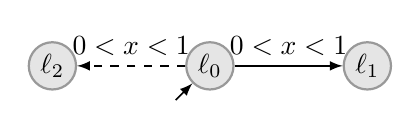
\begin{tikzpicture}[node distance=2cm,auto]
    \tikzstyle{every state}=[minimum size=17pt,inner sep=0pt]
    %\everymath{\scriptstyle}
    \node[state] at (1,0) (A) {$\ell_0$};
    \node[state,right of=A] (B) { $\ell_1$};
    \node[state,left of=A] (C) {$\ell_2$};
    \path[initial] (A.-135) edge +(-135:3mm);
    \path[arrow] 
    (A) edge node[above] {$0<x<1$} (B)
    (A) edge[dashed] node[above] {$0<x < 1$} (C);
  \end{tikzpicture}
  \caption{Timed arena~$\TA_2$. Solid arrow is Eve's, dashed one is Adam's.}
%    \Eve's edges are shown with plain arrows, and \Adam's with dashed ones.}
  \label{10-fig:ta2}
\end{figure}




\begin{example}[Timed Games are not Determined]
  In the timed arena~$\TA_2$ defined in~\cref{10-fig:ta2}, from configuration~$(\ell_0,\vec{0})$, \Eve does not have a winning strategy to reach location~$\ell_1$, but \Adam does not have a winning strategy either to avoid~$\ell_1$.
  In fact, available moves for both players consist in~$(d,(\ell_0,\ell_1))$ with~$0< d<1$ for \Eve, and~$(d',(\ell_0,\ell_2))$ with~$0< d' < 1$ for~\Adam.
  Thus, for any particular delay~$0<d<1$ chosen by~\Eve, \Adam has a possible delay $d<d'<1$ which leads to~$\ell_2$, which is losing for~\Eve.
  This shows that \Eve does not have a winning strategy.
  The argument is however symmetric, and \Adam also does not have a winning strategy to avoid~$\ell_1$.
  Timed games are thus non determined.
\end{example}




%\medskip
%Although the infinite-state concurrent games we defined above
%precisely capture the semantics of timed games we study,




%% \medskip
%% \NM{rewrite}
%% we consider the game~$(\TA,\Omega)$ in the rest of the chapter.
%% In~particular, we~define a~\emph{play} of~$\calT$ as a play of~$\TA$,
%% and a strategy for a player in~$\calT$ as a strategy for the same
%% player in~$\TA$.

%sequence $\rho = q_1q_2\ldots$ where $q_i \in
%V$ with~$q_1 = (\ell_0,\vec{0})$ and 
%such that for each~$i\geq 1$, 
%there exists~$e_i \in E$ and~$d\geq 0$ with $q_{i+1} = \step(q_i,(d,e_i))$.
%A run is \emph{maximal} if it is an infinite sequence or if it ends in
%$V_{\Eve}$ with no possible successor.
%Finite runs are called \emph{histories}.

%We define a~\emph{strategy} for Eve
%as a function~$f\colon V^* \rightarrow \Realnn \times \EE$
%such that for all histories~$q_1q_2\ldots q_k$, $f(q_1q_2\ldots q_k)$
%is a valid move at~$q_k$.

%The set of \emph{outcomes} of the timed game~$\calT$ \emph{from location~$\ell_0$ under
%strategy~$f$} is defined as the set of maximal runs~$\rho$ such that
%\begin{enumerate}
%  \item $\rho_1 = (\ell_0,\vec{0})$,
%  \item for all~$i\geq 1$, either~$q_{i+1} \in \post(q_i,f(q_1q_2\ldots q_i))$
%\end{enumerate}
%We only consider reachability objectives in this chapter. 
%Given a target
%location~$T \in \Locs$, we
%define~$\Omega(T)$ as the set of maximal runs that visit~$T$ at least once.
%A strategy~$f$ for Eve is \emph{winning} if all outcomes under~$f$ belong to~$\Omega(T)$.


\begin{example}[Winning strategy on running example]
Let us consider again the example of \cref{10-fig:ta1} and see whether Eve
has a winning strategy from the initial configuration.
At the initial configuration~$\ell_1,x=0$, \Eve needs to make a move towards~$\ell_2$
while~$x\leq 1$ since whenever~$x>1$, \Adam can move to~$\ell_5$ which guarantees \Eve's lost.
Assume the game proceeds to~$\ell_2$ with any value~$x\leq 1$. Here, \Eve can try to wait
until~$x\geq 2$ and go to~$G$. However, if~$x<1$, then \Adam can move to~$\ell_3$.
From this location, \Eve can guarantee to come back to~$\ell_2$ with~$x=1$, and then move to~$G$ and win the game.
Assume now that from~$\ell_1$, the game proceeds to~$\ell_3$ with~$x=0$ due to~\Adam's move.
Again, \Eve can wait for 1 time unit, and go back to~$\ell_2$ with~$x=1$, and win the game.
%
Hence, \Eve has a winning strategy from $\ell_1$ for all~$x\leq 1$, and from~$\ell_2$
for all values of~$x$.
\end{example}


In this chapter, the main problem we are interested in is determining
whether \Eve has a strategy for her reachability objective.
Let~$\vec{0}$ denote the clock valuation assigning~$0$ to all clocks.

\begin{problem}
  Given a timed arena~$\calT$, initial location~$\ell_0$, and a
  reachability objective~$\Reach(\Win)$,
  decide whether \Eve has a
  winning strategy in~$(\calT,\Reach(\Win))$ from
  configuration~$(\ell_0,\vec{0})$.
\end{problem}

The difficulty of this problem is that the concurrent
game~$((V,E),\Delta,\Omega)$ has an infinite state-space, and players
have infinitely many actions.  We~thus start by studying a data
structure to represent sets of states and operations to compute
successors and predecessors on these sets.  We then give two
algorithms to solve the above problem.  We~also show how such a
strategy for \Eve can be computed and finitely represented.


\section{State-Space Representation}
%%%%%%%%%%%%%%%%%%%%%%%%%%%%%%%%%%%%%%%%%%%%%%%%%%%%%%%%%%%%%%%%%%%%%%
We introduce a data structure to represent sets of clock
valuations and manipulate them efficiently in order to compute
successors and predecessors in a given timed game. This will allow us
to use a fixpoint characterization of the winning states analogous to
that in finite games as in \cref{chap:regular}. %Chapter ...

A~\emph{""zone""} is any subset of~$\Realnn^\Clocks$ that can be defined
using a clock constraint (hence a~zone is convex).  We will see that
sets of states that appear when exploring the state space of a timed
game can be represented using zones.  We~use the
\emph{difference-bound matrices} to represent zones:
this is one of the main data structures used in timed-automata
verification~\cite{Dil90,BM83}. The~idea is to store, in a matrix,
upper bounds on clocks and on differences of pairs of clocks.
%, and an upper bound on the difference of each pair of clocks.
Formally, given a clock
set~$\Clocks=\{x_1,\ldots,x_m\}$, we define $\Clocksz = \Clocks \cup \{x_0\}$
where~$x_0$ is seen as a
special clock which is always~$0$.
%, which is just to simplify the subsequent notations.
A~""difference-bound matrix""~(""DBM"") is a $|\Clocksz|\times |\Clocksz|$
matrix with coefficients in $\{\mathord\leq,\mathord<\} \times
\mathbb{Z}$.  For any DBM~$M$, the $(i,j)$-component of the matrix~$M$
will be written $(\prec^M_{i,j}, M_{i,j})$ where $\prec^M_{i,j}$ is
the inequality in~$\{\mathord\leq,\mathord<\}$, and $M_{i,j}$ the
integer coefficient. A~DBM~$M$ defines the zone
%~$[M]$ described by
%the following clock constraints
\[
  [M] = \Bigl\{v\in \Realnn^{\Clocks}\Bigm|
  \bigwedge_{0\leq i,j \leq |\Clocksz|} v(x_i)-v(x_j) \prec^M_{i,j} M_{i,j}\Bigr\},
\]
where $v(x_0) = 0$.

\begin{example}
  Consider the clock set $\Clocks=\{x_1,x_2\}$
  and the zone $Z$ defined by 
  $x_1\leq 1 \land x_1-x_2 \leq 0 \land x_2\leq 3\land x_2-x_1 \leq 2$, which can be
  written as the following DBM:
  \[
    M=\begin{pmatrix}
      (\leq,0) &(\leq,0) &(\leq,0)\\
      (\leq,1) &(\leq,0) &(\leq,0)\\
      (\leq,3) &(\leq,2) &(\leq,0)
    \end{pmatrix}
    \qquad
  \tikz[scale=.45]{ 
    \path[use as bounding box] (-1,1.2) -- (2,4);
    \begin{scope}
      \draw[latex'-latex'] (3.5,0) node[right] {$x_1$}
        -| (0,3.8) node[left] {$x_2$};
      \begin{scope}
        \path[clip] (0,0) -- (3.5,0) [rounded corners=12mm]
          -- (3.5,3.9) [rounded corners=0mm] -| (0,0);
        \draw[dgrey,fillarea] (0,0) -- (1,1) |- (0,3) -- cycle;
        \begin{scope}[opacity=.3]
          \foreach \x in {-4,...,4}
                 {\draw (\x,0) -- +(9,9);
                   \draw (0,\x) -- +(9,0);
                   \draw (\x,0) -- +(0,9);}
        \end{scope}
        %\draw[line width=.6pt,opacity=.8] (0,0) -- (1,1) |- (0,3) -- cycle;
      \end{scope}
    \end{scope}
    %% \path[use as bounding box] (-1,0.5) -- (2,1.5);
    %% \begin{scope}[scale=.4]
    %%   \fill[gray] (0,0) -- (1,1) -- (1,3) -- (0,2) -- cycle;
    %%   \draw[-latex',line width=.6pt] (0,0) -- (3.5,0) node[right] {$x_1$};
    %%   \draw[-latex',line width=.6pt] (0,0) -- (0,3.5) node[left] {$x_2$};
    %%   \begin{scope}[line width=0.1pt]
    %%   \draw[-] (1,0) -- (1,3.5);
    %%   \draw[-] (2,0) -- (2,3.5);
    %%   \draw[-] (0,1) -- (3.5,1);
    %%   \draw[-] (0,2) -- (3.5,2);
    %%   \draw[-] (0,0) -- (3.5,3.5);
    %%   \draw[-] (1,0) -- (3.5,2.5);
    %%   \draw[-] (2,0) -- (3.5,1.5);
    %%   \draw[-] (0,1) -- (2.5,3.5);
    %%   \draw[-] (0,2) -- (1.5,3.5);
    %% \end{scope}
    %% \end{scope}
    }
  \]
%Note for instance that the coefficient~$3$ on the third row and
%  first column
  For instance, $M[2,0]=(\leq, 3)$ represents the
  constraint~$x_2-x_0\leq 3$, i.e., $x_2\leq 3$.
%  corresponds to $x_2 - x_0 \leq 3$, which is equivalent to $x_2 \leq 3$.
%  The~subset of~$\Realnn^2$ represented by this DBM is represented on
%  the diagram.
  The~diagram to the right of the figure represents the set~$[M]$.
\end{example}

We now define elementary operations on DBMs which are used to explore
the state space of timed games. We start by giving set-theoretic
definitions and then comment on their computation with~DBMs.

Let $\posttime(Z)$ denote the zone describing the
\emph{time-successors} of~$Z$, and~$\pretime(Z)$ the
\emph{time-predecessors} of~$Z$. Formally,
\begin{xalignat*}1
    \posttime(Z)&= \{v \in \Realnn^{\Clocks}
    \mid \exists t\geq 0.\  v-t \in Z\}
    \\
    \pretime(Z) &=
    \{v \in \Realnn^{\Clocks} \mid \exists t \geq 0.\ v + t \in Z\}.
\end{xalignat*}

Given~$R\subseteq\Clocks$, we also define
\begin{xalignat*}1
  \reset_R(Z) &= \{v \in \Realnn^{\Clocks} \mid \exists v' \in Z.\
  v=v'[R\leftarrow 0]\} \\
  \unreset_R(Z) &= \{ v \in \Realnn^{\Clocks} \mid \exists v' \in Z.\
  v' = v[R \leftarrow 0]\}.
\end{xalignat*}
%Notice that~$\freeta_R$ is the inverse of~$\reset_R$.
%Intersection is denoted $Z \cap Z'$.

These operations, together with intersection, suffice to describe
one-step successors and predecessors by an edge of a timed automaton.
For instance, given edge~$e=(\ell,g,R,\ell')$ and
set~$S \subseteq \Realnn^\Clocks$, the~set of states that are reached
after letting time elapse and taking edge~$e$ can be obtained as
% \[
%   \begin{array}{rl}
%     \postta_e(S) = \{ (\ell',\nu') &\mid \exists (\ell,\nu) \in S, \nu \models g, \exists d\geq
%                                    0,~\nu' = \nu[R\leftarrow 0] + d\}.
%   \end{array}
% \]
% If~$G$ denotes the zone corresponding to the guard~$g$, then we 
%have~$\postta_e(S) = \posttime((S \cap G)[R\leftarrow 0])$.
\[
  \postta_e(S) = \reset_R(\posttime(S)\cap G),
\]
where~$G$ denotes the zone corresponding to the guard~$g$.
Similarly, we can compute the predecessors of~$S$ by edge~$e$ as
\[
\preta_e(S) = \pretime(G \cap \unreset_R(S)).
% \cap (\bigwedge_{x \in R}x=0)),
\]
%which is the set of states which, after a delay, satisfy~$g$ and end
%in~$S$ by resetting~$R$.
We~illustrate these constructions on \cref{10-fig:opzones}.
\begin{figure}[ht]
  \centering
  \begin{tikzpicture}[scale=.45]
    \begin{scope}
      \draw[latex'-latex'] (4.5,0) node[right] {$x_1$}
        -| (0,4.5) node[left] {$x_2$};
      \begin{scope}
        \path[clip] (0,0) -- (4.5,0) [rounded corners=12mm]
          -- (4.5,4.5) [rounded corners=0mm] -| (0,0);
        \fill[dgrey,fillarea] (1,1) -- (2,2) |- (1,3) -- cycle;
        %\draw[line width=.6pt,opacity=.8] (1,1) -- (2,2) |- (1,3) -- cycle;
        \fill[opacity=.6,dgrey,hatcharea] (1,1) -- (5,5) -| cycle;
        %\draw[line width=.6pt,opacity=.8] (1,1) -- (5,5) -| cycle;
        \begin{scope}[opacity=.3]
          \foreach \x in {-4,...,4}
                 {\draw (\x,0) -- +(9,9);
                   \draw (0,\x) -- +(9,0);
                   \draw (\x,0) -- +(0,9);}
        \end{scope}
      \end{scope}
      \path (3,0.5) node (Z) {$Z$} edge[-latex',bend left=20] (1.6,1.4);
      \path (4,1.5) node (Y) {$\posttime(Z)$} edge[-latex',bend right=20] (2.9,2.7);
    \end{scope}
    %%
    \begin{scope}[xshift=6.5cm]
      \draw[latex'-latex'] (4.5,0) node[right] {$x_1$}
        -| (0,4.5) node[left] {$x_2$};
      \begin{scope}
        \path[clip] (0,0) -- (4.5,0) [rounded corners=12mm]
          -- (4.5,4.5) [rounded corners=0mm] -| (0,0);
        \fill[dgrey,fillarea] (1,1) -- (2,2) |- (1,3) -- cycle;
        \fill[opacity=.6,dgrey,hatcharea] (0,0) -- (2,2) |- (1,3) -- (0,2) -- cycle;
        %\draw[line width=.6pt,opacity=.8]  (0,0) -- (2,2) |- (1,3) -- (0,2) -- cycle;
        %\draw[line width=.6pt,opacity=.8] (1,1) -- (2,2) |- (1,3) -- cycle;
          \begin{scope}[opacity=.3]
            \foreach \x in {-4,...,4}
                 {\draw (\x,0) -- +(9,9);
                   \draw (0,\x) -- +(9,0);
                   \draw (\x,0) -- +(0,9);}
          \end{scope}
      \end{scope}
      \path (3,1.5) node (Z) {$Z$} edge[-latex',bend right] (2.1,2.6);
      \path (3.5,0.5) node (Y) {$\pretime(Z)$} edge[-latex',bend left=10] (.6,0.5);
    \end{scope}
    %%
    \begin{scope}[xshift=13cm]
      \draw[latex'-latex'] (4.5,0) node[right] {$x_1$}
        -| (0,4.5) node[left] {$x_2$};
      \begin{scope}
        \path[clip] (0,0) -- (4.5,0) [rounded corners=12mm]
          -- (4.5,4.5) [rounded corners=0mm] -| (0,0);
        \fill[dgrey,fillarea] (1,1) -- (2,2) |- (1,3) -- cycle;
        %\draw[line width=.6pt,opacity=.8] (1,1) -- (2,2) |- (1,3) -- cycle;
        \draw[line width=3.2pt,dgrey] (1,0) -- (2,0);
        \begin{scope}[opacity=.3]
          \foreach \x in {-4,...,4}
                 {\draw (\x,0) -- +(9,9);
                   \draw (0,\x) -- +(9,0);
                   \draw (\x,0) -- +(0,9);}
          \end{scope}
      \end{scope}
      \path (3.2,1.8) node (Z) {$Z$} edge[-latex',bend right] (2.1,2.6);
      \path (3.5,0.8) node (Y) {$\reset_{x_2}(Z)$} edge[-latex',bend right=20] (1.4,0.1);
    \end{scope}
    %%
    \begin{scope}[xshift=19.5cm]
      \draw[latex'-latex'] (4.5,0) node[right] {$x_1$}
        -| (0,4.5) node[left] {$x_2$};
      \begin{scope}
        \path[clip] (0,0) -- (4.5,0) [rounded corners=12mm]
          -- (4.5,4.5) [rounded corners=0mm] -| (0,0);
        \fill[dgrey,fillarea] (1,0) -- (2,0) -- (3,1) |- (2,3) -- (1,2) -- cycle;
        %\draw[line width=.6pt,opacity=.8] (1,0) -- (2,0) -- (3,1) |- (2,3) -- (1,2) -- cycle;
        \fill[opacity=.6,dgrey,hatcharea] (1,5) -| (2,0) -| cycle;
        %\draw[line width=.6pt,opacity=.8]  (1,5) -| (2,0) -| cycle;
        \begin{scope}[opacity=.3]
          \foreach \x in {-4,...,4}
                 {\draw (\x,0) -- +(9,9);
                   \draw (0,\x) -- +(9,0);
                   \draw (\x,0) -- +(0,9);}
        \end{scope}
      \end{scope}
      \path (5,1.5) node (Z) {$Z$} edge[-latex',bend right] (3.1,2.6);
      \path (3.9,4) node (Y) {$\unreset_{x_2}(Z)$} edge[-latex',bend left=12] (2.1,3.4);
    \end{scope}
        
  \end{tikzpicture}
  \caption{Operations on zones}\label{10-fig:opzones}
\end{figure}

It is not hard to prove that the above operations preserve zones: if~$S$ is a
zone, then so is the result of any of these operations. Moreover, each
single operation can be computed in time~$O(|\Clocks|^3)$ using the
DBM representation. The~underlying algorithms often modify some
elements of the matrix and run an all-pairs shortest path algorithm,
namely the Floyd-Roy-Warshall algorithm, on a graph whose adjacency
matrix is the given~DBM.  Computing the shortest paths renders the DBM
\emph{canonical}; in~fact, this allows one to compute the tightest
constraints on all differences of clock pairs, and this can be shown
to yield a unique representation of a given zone.

Let us call the above operations \emph{basic operations} on DBMs~\cite{BY04}.
%\NM{add refs}
\begin{theorem}
  Given a DBM of size~$n\times n$, any basic operation yields a DBM
  and can be computed in time~$O(n^3)$.
\end{theorem}

% \[
%   \begin{array}{rl}
%     \preta_e(S) = \{ (\ell,\nu) &\mid \nu \models g, \exists d\geq 0, \nu[R\leftarrow 0]+d \in S \},
%   \end{array}
% \]
% which can be defined by~$\post_e(S) = 

% We already defined the controllable predecessor operator in the previous
% section. Another basic operation often used in verification and synthesis is the
% successor computation. Given a set of states~$S$, and edge~$e$, let us define the set of
% states that can be reached by taking the edge~$e=(\ell,g,a,R,\ell')$ and then delaying as follows.
% \[
%   \begin{array}{rl}
%   \post_e(S) = \{ (\ell',\nu') &\mid (\ell,\nu) \in S, \nu \models g, \exists d\geq
%   0, \\&~\nu' = \nu[R\leftarrow 0] + d\}.
% \end{array}
% \]

Observe that a DBM always describes a convex subset
of~$\Realnn^\Clocks$ since it is a conjunction of convex clock
constraints. However, the set of winning states is in general
non-convex in timed games. The~simple arena
of~\cref{10-fig:non-convex} provides an example: if~\Eve's objective
is to reach~$\ell_1$, then it should just avoid the configurations
satisfying~$1\leq x_1,x_2\leq 2$. But this set of predecessors is then
non-convex as shown in~\cref{10-fig:non-convex}.
%example. Assume there are only controllable edges from location~$\ell$
%to~$\ell_1$ and~$\ell_2$ with disjoint guards, with no resets, and that the
%objective is to reach~$\ell_1$ or~$\ell_2$.
%%Then the figure
%on the right shows the set of states from which Eve can delay and
%reach either~$\ell_1$ or~$\ell_2$ to satisfy her objective.
We~thus have to work with unions of zones, also called
\emph{""federations""} of zones, or \emph{federations} for~short.

\begin{figure}[ht]
  \centering
  \begin{tikzpicture}[node distance=2.5cm,auto]
%    \tikzstyle{every state}=[minimum size=17pt,inner sep=0pt]
%    \path[use as bounding box] (-2,-1) -- (2,0);
    %\everymath{\scriptstyle}
    \node[state] at (0,0) (A) {$\ell$};
    \draw[initial] (A.-135) -- +(-135:3mm);
    \node[state,double] at (2.5,0) (B) {$\ell_1$};
    \node[state] at (-2.5,0) (C) {$\ell_2$};
    \path[arrow] 
    (A) edge node[above] {$\genfrac{}{}{0pt}{0}{-2 \leq x_1-x_2 \leq 1}{{}\wedge x_2 \leq 3}$} (B)
    (A) edge[dashed] node[above] {$1\leq x_1,x_2 \leq 2$} (C);
    %
    \begin{scope}[xshift=4cm,yshift=-1cm,scale=.45]
      \draw[latex'-latex'] (4.5,0) node[right] {$x_1$}
        -| (0,4.5) node[left] {$x_2$};
      \begin{scope}
        \path[clip] (0,0) -- (4.5,0) [rounded corners=12mm]
          -- (4.5,4.5) [rounded corners=0mm] -| (0,0);
        \fill[dgrey,fillarea] (1,0) -- (2,1) -| (1,2) -| (2,1) -- (4,3) -- (1,3) -- (0,2) |- cycle;
          \begin{scope}[opacity=.3]
            \foreach \x in {-4,...,4}
                 {\draw (\x,0) -- +(9,9);
                   \draw (0,\x) -- +(9,0);
                   \draw (\x,0) -- +(0,9);}
          \end{scope}
      \end{scope}
%      \path (3,0.5) node (Z) {$Z$} edge[-latex',bend left=20] (1.6,1.4);
%      \path (4,1.5) node (Y) {$\posttime(Z)$} edge[-latex',bend right=20] (2.9,2.7);
    \end{scope}
%%     \begin{scope}[scale=.4]
%%       \fill[gray] (0,0) -- (0,1) -- (1,2) -- (1,1) -- 
%%       (2,1) -- (1,0) -- cycle;
%%       \fill[gray] (2,1) -- (2,2) -- (1,2) -- (2,3) -- 
%%       (4,3);
%%       %(3.2,3.2) -- (3.2,2.2) -- (2.2,1.2);

%% %      \fill[gray] (0,2) -- (1,2) -- (1,3.2) -- (0,3.2) -- cycle;
%% %      \fill[gray] (0,1) -- (1,2) -- (0,2) -- cycle;
%% %      \fill[gray] (2,0) -- (2,1) -- (3.2,1) -- (3.2,0) -- cycle;
%% %      \fill[gray] (1,0) -- (2,1) -- (2,0) -- cycle;
%%       \draw[-latex',line width=.6pt] (0,0) -- (4.5,0) node[right] {$x$};
%%       \draw[-latex',line width=.6pt] (0,0) -- (0,4.5) node[left] {$y$};
%%       \begin{scope}[line width=0.1pt]
%%         \draw[-] (1,0) -- (1,4);
%%         \draw[-] (2,0) -- (2,4);
%%         \draw[-] (3,0) -- (3,4);
%%         \draw[-] (4,0) -- (4,4);
%%         \draw[-] (0,1) -- (4,1);
%%         \draw[-] (0,2) -- (4,2);
%%         \draw[-] (0,3) -- (4,3);
%%         \draw[-] (0,4) -- (4,4);
%%         \draw[-] (0,0) -- (4,4);
%%         \draw[-] (1,0) -- (4,3);
%%         \draw[-] (2,0) -- (4,2);
%%         \draw[-] (0,1) -- (3,4);
%%         \draw[-] (0,2) -- (2,4);
%%       \end{scope}
%%     \end{scope}
  \end{tikzpicture}
  \caption{Winning configurations (in~$\ell$)
    for~\Eve to ensure reaching~$\ell_1$.
% in one step is non-convex and shown on the right.
  }
  \label{10-fig:non-convex}
\end{figure}

One particular operation that we need is complementation.
The~complement of a convex set is of course not convex in general, but
we can still compute, in polynomial time, the complement of a DBM~$M$,
written~$M^c$, as a federation of~DBMs.
\begin{theorem}
  The complement of a DBM of size~$n\times n$ can be computed as a
  federation of at most~$n(n-1)$ DBMs.
%\footnote{I think it suffices to invert each component, without reducing afterwards. Check this.}
\end{theorem}
The above theorem is seen easily as follows. Since a DBM represents a
conjunction of constraints, the complement is computed easily as the
disjunction of the complement of each elementary constraint appearing
in~it.  For~instance, the~complement of $x_1\leq 1 \land x_2 \geq 2$ is
$x_1>1 \lor x_2<2$, which can be represented as the federation of two
zones.



%\section{Algorithms}

In the rest of this chapter, we describe two algorithms to solve timed
games using the DBM data structure and the operations introduced
above. Our~algorithms are extensions of those used for finite games,
but we explore the set of zones instead of the set of vertices, and
predecessor and successor operations are replaced by their zone-based
counterparts.

As for finite games, we are interested in computing a fixpoint to
determine whether a given configuration is winning for~\Eve. We~start
by introducing the zone-based counterparts of the controllable predecessors operator
which
is the main tool in the algorithms.

\section{Controllable-Predecessor Operator}
%%%%%%%%%%%%%%%%%%%%%%%%%%%%%%%%%%%%%%%%%%%%%%%%%%%%%%%%%%%%%%%%%%%%%%
%\OS{We might rather call this attractor}
%\NM{Pour moi, ``controllable pred.'' est en 1 pas, et ``attractor'' est le point fixe. Mais on peut en discuter}
%Present this operator with examples as the main tool of the
%subsequent algorithms.  We are going to follow the algorithm for the
%finite-state case and define controllable predecessors, but this
%needs some care due to delay transitions in timed automata.
% Due to the-real-time and concurrent nature of our formalism, we need
% to define a particular predecessor operator that takes time delays
% into account.

We present the controllable-predecessor operator which, given sets of
states $X$ and~$Y$, returns the set of states from which \Eve can
reach~$X$ in one step, while avoiding states of~$Y$ during \Eve's
delay. Intuitively, the states in~$Y$ are the states from which \Adam
may force an action leading outside of~$X$, which \Eve would better avoid.

%\OS{This operations make sense with the concurrent semantics...}
Recall that $\vertices = \Locs \times \Realnn^\Clocks$.
The set of \emph{""safe time-predecessors""} to reach~$X \subseteq \vertices$ while
avoiding~$Y \subseteq \vertices$
%\NM{$\VE$ or $V$?}
is defined as follows:
%\[
%  \begin{array}{ll}
\begin{multline*}
\predt(X,Y) = \{(\ell,\nu) \in \vertices \mid \exists d\geq
    0.\ (\ell,\nu+d) \in X \wedge{} \\
    \forall d' \in[0,d).\ (\ell,\nu+d') \not  \in Y\}.
\end{multline*}
%  \end{array}
%\]
In words, from any configuration of $\predt(X,Y)$,
the set~$X$ can be reached by
delaying while never crossing any configuration of~$Y$ on the way. 
For any $X \subseteq \vertices$, let us denote
\[
  \predc(X) = \{ (\ell,\nu) \in \vertices \mid \exists e \in \EE(\ell).\ 
\exists (\ell',\nu') \in X.\ (\ell,\nu) \xrightarrow{e} (\ell',\nu')\}.
\]
This is the set of immediate predecessors of~$X$ by edges in~$\EE$.
Symmetrically, we~define $\predu(X)$ using~$\EA$ instead of~$\EE$.
Our controllable-predecessor operator is then defined as 
%
%\NM{Replace $\predc(X)$ with $X\cup\predc(X)$? besoin dans une preuve, je crois. A verifier}
%\NM{C'est bien X cup predc(X) dans le papier [BCF+05]. J'ai corrig\'e}
\[
  \pi(X) = \predt(X\cup \predc(X), \predu(\vertices \setminus X)).
\]

%\NM{!!! Cette approche necessite la semantique ``jeux concurrents''.
%  Reecrire avec jeux concurrents + ajouter remarque ``jeux a tours''}
%\NM{$\calQ$ undefined}
Intuitively, the states in~$\pi(X)$ are those from which \Eve~can wait
until she
can take a controllable transition to~reach~$X$, and so that
%any uncontrollable transition that might happen while waiting remains
%inside~$X$.
no transitions that \Adam could take while \Eve is waiting may lead
outside of~$X$.

\begin{lemma}\label{10-lem:pimonotonic}
  The operator $\pi$ is %non-decreasing
  order-preserving: if~$X\subseteq Y$, then
  $\pi(X) \subseteq \pi(Y)$.  %\NM{useful later}
\end{lemma}

\begin{example}
Consider the timed game to the left of
\cref{10-fig:contpred}. In~that game, \Eve can reach her target when
clock~$x_2$ reaches value~$3$ while~$x_1$ is in~$[1;4]$. However,
\Adam can take the game to a bad state when simultaneously
$x_1\in[1;2]$ and $x_2\leq 2$. The~diagram to the right of
\cref{10-fig:contpred} shows the set of winning valuations for~\Eve:
it~is computed as $\predt(X,Y)$ where $X=\predc(\{W\}\times\Realnn)$
and $Y=\predu(\{\ell_0,\ell_1\}\times\Realnn)$.

\begin{figure}[h]
  \centering
  \begin{tikzpicture}
    \draw (0,1) node[state] (a) {$\ell_0$};
    \draw (0,-1) node[state] (b) {$\ell_1$};
    \draw (3,0) node[state,double] (W) {$W$};
    \draw[arrow] (a) -- (W) node[midway,above right] {$\genfrac{}{}{0pt}{0}{1\leq x_1\leq 4}{{}\wedge x_2=3}$};
    \draw (a) edge[arrow,dashed] (b) node[midway,left] {$\genfrac{}{}{0pt}{0}{1\leq x_1\leq 2}{{}\wedge x_2\leq 2}$};
    \draw[initial] (a.135) -- +(135:3mm);
    %
    %
    \begin{scope}[xshift=5cm,yshift=-1cm,scale=.55]
      \draw[latex'-latex'] (4.5,0) node[right] {$x_1$}
      -| (0,4.5) node[left] {$x_2$};
      \begin{scope}
        \path[clip] (0,0) -- (4.5,0) [rounded corners=10mm]
          -- (4.5,4.5) [rounded corners=0mm] -| (0,0);
        \fill[opacity=.6,dgrey,hatcharea] (1,0) -| (2,2) -| cycle;
        %\draw[line width=1pt,black,opacity=1] (1,0) -| (2,2) -| cycle;
        \fill[dgrey,fillarea] (0,1) -- (1,2) -| (2,1) -- (4,3) -- (1,3) -- (0,2) -- cycle;
        \draw[line width=3.2pt,dgrey] (1,3) -- (4,3);
        \begin{scope}[opacity=.3]
        \foreach \x in {-4,...,4}
                 {\draw (\x,0) -- +(9,9);
                   \draw (0,\x) -- +(9,0);
                   \draw (\x,0) -- +(0,9);}
        \end{scope}
      \end{scope}
%      \path (3,0.5) node (Z) {$Z$} edge[-latex',bend left=20] (1.6,1.4);
%      \path (4,1.5) node (Y) {$\posttime(Z)$} edge[-latex',bend right=20] (2.9,2.7);
      \path (3.5,4) node {$X$} edge[-latex',bend right=12] (2.8,3.2);
      \path (3.5,0.5) node {$Y$} edge[-latex',bend left=12] (2.2,0.6);
      \path (4.5,1.5) node {$\pi(W)$} edge[-latex',bend left=12] (2.6,1.8);
    \end{scope}
  \end{tikzpicture}
  \caption{Controllable predecessors}\label{10-fig:contpred}
\end{figure}
\end{example}
% \begin{lemma}
%   Consider a timed arena~$\calT$.
%   For any~$X \subseteq V$,  %%\mathbb{R}_{\geq 0}^\Clocks$,
%   %%\NM{il faut $X \subseteq \Locs\times \mathbb{R}_{\geq 0}^\Clocks$?}
%   and any configuration~${q \in \vertices}$, it~holds $q \in \pi(X)$ if, and only~if
%   $q \in \mathsf{Attr}(X)$.
% \end{lemma}
% \NM{!!  l'attracteur correspond au point fixe. + enoncer ``$\pi(X)=\mathsf{Attr}(X)$''}

% \begin{proof}
%   .... \NM{(re)definir $\textsf{Attr}_\TA(X)$? Mettre ref section 2.1 ?}
% \end{proof}

% The following theorem is the fixpoint characterization of the winning states
% for~$\Eve$. It is the timed automata analogue to Theorem ....
% \begin{theorem}
%   \label{10-thm:fp}
%   Given a timed game~$(\calT,\Omega)$ with a reachability objective~$\Omega$,
%   a configuration~$q$ is winning for~$\Eve$ if, and only if
%   there exists~$X \subseteq \mathbb{R}_{\geq 0}^\Clocks$ such that
%   $q \in X$ and~$X = \pi(X)$.
%   \NM{Il faut prendre le plus petit pt fixe (sinon $X=\Locs\times\Realnn^{\Clocks}$ convient)}
% \end{theorem}



\begin{remark}
  When considering zero-sum objectives (which we do in this chapter),
a~turn-based arena can be built to decide whether \Eve has a winning
strategy (and~possibly construct~one).  Intuitively, the turn-based
arena is obtained by letting \Eve first pick a pair~$(d,e)$ with~$e
\in \EE$, and then letting \Adam either respect this choice (i.e.,
play a larger delay) or preempt \Eve's action by choosing $(d',e')$
with~$d' \leq d$ and~$e' \in \EA$.
\Eve has a winning strategy in this turn-based arena if, and only if she has one in the original game.
However, this does not apply to \Adam; if he has a winning strategy, this only means that \Eve
does not have a winning strategy in the original game.

%\paragraph{Turn-Based Game Semantics}
Given~$\calT = (\Locs, \Clocks,\EE,\EA, c)$, we define the arena~$\TA
= (\vertices,\VE,\VA,E, c'')$ 
with objective~$\Omega$, where~$\VE = \Locs\times \Realnn^\Clocks$ and
$\VA=\Locs\times\Realnn^\Clocks\times(\Realnn \times \EE
\cup\{\bot\})$.  The~set of successors of configuration~$(\ell,\nu)
\in \VE$ is the set $\{(\ell,\nu,a)\mid a \text{ available at
}(\ell,\nu)\}$.
%  \[
%  \{ (\ell,\nu,(d,e)) \mid e \text{ valid at } \nu+d\},
%  \]
From a configuration~$((\ell,\nu),(d,e))\in\VA$, several cases may
occur:
%\todo{OS: Rephrased. Please check}
\begin{itemize}
\item if \Adam has no available action from~$(\ell,\nu)$, or if he can
  only play actions~$(d',e')$ with $d'>d$, then the only transition
  from~$((\ell,\nu),(d,e))$ goes to $\step((\ell,\nu),(d,e))$;
\item Otherwise, for all actions~$(d',e')$ for \Adam satisfying $d'\leq d$,
  there is a transition from~$((\ell,\nu),(d,e))$
  to $\step((\ell,\nu),(d',e'))$.
  Moreover, if \Adam has an available action~$(d',e')$ with~$d'\geq d$,
  then there is also a transition
  from~$((\ell,\nu),(d,e))$ to $\step((\ell,\nu),(d,e))$.
% \item if \Adam can play an action~$(d',e')$ with $d'\leq d$, then
%   there is a transition from~$((\ell,\nu),(d,e))$
%   to $\step((\ell,\nu),(d',e'))$.
\end{itemize}
%\[
%  \{\step((\ell,\nu),(d,e))\}
%  \cup
%  \{ (\step((\ell,\nu), (d',e')) \mid d' \leq d, e' \in \EA(\ell), e'+d' \models g_{e'}\}.
%\]
From a configuration~$((\ell,\nu),\bot)$, there is a transition
to~$\step((\ell,\nu),(d',e'))$ for each available action~$(d',e')$
of~\Adam.
The coloring function is defined as~$c''((\ell,\nu)) = c(\ell)$
and~$c''((\ell,\nu),(d,e)) = c(\ell)$.
%The function~$\Delta$ is defined so that it induces a bijection between actions
%and the above edges for each player. We do not need its precise definition
%since we will directly refer to edges.


\end{remark}



\section{Backward Algorithm}
%%%%%%%%%%%%%%%%%%%%%%%%%%%%%%%%%%%%%%%%%%%%%%%%%%%%%%%%%%%%%%%%%%%%%%
%From~\cref{10-thm:fp}, and
Given the DBM data structure we presented,
a backward fixpoint algorithm follows for computing the winning configurations in a timed game:

\begin{theorem}
   \label{10-thm:timed-control}
   For any timed game~$\TA$ and target set~$G \subseteq \VE$, 
   the~limit $\lim_{k \rightarrow \infty} \pi^k(G)$ exists, and is reached 
   in a finite number of steps. This limit is precisely the set of states from
   which the controller has a winning strategy for reaching~$G$.
\end{theorem}

\begin{proof}[Sketch]
%Not immediate: Why does the fixpoint terminate here?
  We~briefly explain why the fixpoint computation terminates and refer
  to~\cite{AMPS98,CDFLL05} for more details.  The~proof relies on the notion of
  \emph{regions}. Intuitively, regions are minimal zones, not
  containing any other zone. More precisely, writing~$K$ for the maximal
  (absolute) integer constant appearing in the timed game, the~set of regions is
  the set of zones associated with
  DBMs~$(\mathord\prec_{i,j},M_{i,j})$ such that
  %\NM{verifier que c'est    ok...}
  \begin{itemize}
  \item $M_{i,j}\in [-K; K]\cup\{-\infty;+\infty\}$ for all~$i$ and~$j$;
  \item for all~$i\not=j$,
     \begin{itemize}
    \item either $M_{i,j}=-M_{j,i}$ and
      $\mathord\prec_{i,j}=\mathord\prec_{j,i}=\mathord\leq$,
     \item or $|M_{i,j}+M_{j,i}|=1$ and 
      $\mathord\prec_{i,j}=\mathord\prec_{j,i}=\mathord<$,
    \item or $(\prec_{i,j},M_{i,j})=(<,+\infty)$ and $(\prec_{j,i},M_{j,i})=(<,-K)$.
     \end{itemize}
  %\todo{Il y a un QED en plein milieu de la preuve...}
  % probleme global avec les QED, on regardera plus tard
  \end{itemize}
  The set of regions form a finite partition of~$\Realnn^{\Clocks}$.
  The~main argument for the proof is that the
  image by~$\pi$ of any finite union of regions is a finite union of
  regions. Since~$\pi$ is non-decreasing, the~sequence~$\pi^k(G)$
  converges after finitely many steps.

  The~fact that $\pi^k(G)$ may
  only contain winning configurations follows from our construction,
  and can be proved easily by induction on~$k$.
  One can also show that for all configurations outside of~$\pi^k(G)$,
  there is no strategy that is winning within~$k$ steps. This follows since
  the definition of~$\pi(\cdot)$ gives the actions to be played by \Adam to
  prevent \Eve from winning.
  Note that this does not necessarily yield a winning strategy for \Adam,
  since the game is not determined.
\end{proof}

%Add more comments.
%Hence, this operator allows us to express the states that can be controlled
%within one step. The following theorem shows that the greatest fixpoint of this
%operator exists and can be computed. 
%This should follow from~\cite{AMPS98,AMP-concur98}.
%See also Tripakis et al. before 2005.


\section{Forward Algorithm}
%%%%%%%%%%%%%%%%%%%%%%%%%%%%%%%%%%%%%%%%%%%%%%%%%%%%%%%%%%%%%%%%%%%%%%
%This is the main development of this section. CONCUR'05.
%
%Present the finite-state version (Liu, Smolka).
%Illustrate it on an example.


The backward algorithm we just presented is conceptually simple, but
it~is often not very efficient in practice,
as federations tend to grow too much in size in each iteration of the
computation.
The forward algorithm we will now present is more efficient in practice.
It performs a forward exploration and only applies the controllable predecessor along branches
that actually reach the target state from the initial state. If the witness
trace is not excessively long, which is often the case in practice,
this limits the size of the federations.
%In finite-state systems, this algorithm is known to find small fixpoints

%When dealing with timed systems, backwards algorithms are easy to
%develop and implement, but they are usually not very efficient in
%practice.
%\NM{Give intuition why? Especially, why for timed games?? La
%  justification donnee dans [Cassez, FORMATS 2007] n'est pas hyper
%  convaincante...}
%As~for solving reachability in timed automata, forward algorithms have
%been designed to gain in efficiency.

We present below the algorithm proposed in~\cite{CDFLL05},
and as a first step, we explain the untimed version of that algorithm,
based on an algorithm of Liu and Smolka for computing
fixpoints~\cite{LS98}.


\subsection*{A Forward Algorithm for Finite-State Games}
%Give the full proof.

The original algorithm of Liu and Smolka is expressed in terms of
\emph{(pre-)fixpoints} in \emph{dependency graphs}: a~dependency graph
is a pair~$G=(V,E)$ in which $E \subseteq V \times 2^V$ relates
states with sets of states.
%
For any order-preserving 
function~$f\colon 2^V\to2^V$
(\emph{order-preserving} meaning non-decreasing for the $\subseteq$-relation),
%\todo{Define order-preserving}
a~\emph{pre-fixpoint} is a set~$X\subseteq V$ for which $f(X)\subseteq
X$; it~is a \emph{fixpoint} if $f(X)=X$. By~Knaster-Tarski theorem, such
functions always admit a least pre-fixpoint which is also the least fixpoint.
% Observe that the least
%pre-fixpoint and the least fixpoint coincide.
%

Fix a dependency graph~$G=(V,E)$. 
For~$W\subseteq V$,
we~define a mapping $f_W\colon 2^V\to 2^V$: for
each~$X\subseteq V$, we~let $f_W(X)=W\cup \{v\in V\mid \exists (v,Y)\in
E.\ Y\subseteq X\}$.
%
%By~Knaster-Tarski theorem, $f_W$~admits a least
%pre-fixpoint, which is also its least
%fixpoint.
Clearly, $X\subseteq X'$ implies $f_W(X)\subseteq f_W(X')$, so that $f_W$ admits
a least (pre-)fixpoint.
The~Liu-Smolka
algorithm aims at deciding whether a given vertex~$v_0\in V$ belongs
to the least fixpoint of~$f_W$.  Classical algorithms for computing
least fixpoints consist in iteratively
computing~$(f_W^i(\emptyset))_i$ until convergence (assuming~$V$~is
finite). Observe that this corresponds to the algorithm of \cref{10-thm:timed-control}
for timed games.
The~Liu-Smolka algorithm proceeds from~$v_0$, and explores
the dependency graph until it can claim that~$v_0$~is, or that it
is~not, in the least fixpoint of~$f_W$.


Before tackling the algorithm, let us link least fixpoints in
dependency graphs and winning sets in concurrent games (with
reachability objectives): with a concurrent arena
$\calC=(V,\Act,\delta,c')$ and a target set~$\Win$, we~associate
the dependency graph $G=(V,E)$, where $(v,T)\in E$ whenever $v\in V$
and $T\subseteq V$ is such that there exists an action~$a$ for which
$T=\{v' \mid \exists a'\in\Act.\ v'=\delta(v,a,a')\}$.  Then for any
set~$X\subseteq V$, the~set~$f_{\Win}(X)$ contains $\Win$ and all the
states from which Eve can force a visit to~$X$ in one step.
We~then~have:
\begin{proposition}\label{10-prop:fixp-game}
The least fixpoint of~$f_{\Win}$ in~$G$ corresponds to the set~$W$ of
winning states for~\Eve in~$\calC$.
\end{proposition}

\begin{proof}
  The winning states of~\Eve form a pre-fixpoint of~$f_{\Win}$
  containing~\Win: indeed, for any~$v\in f_{\Win}(W)$, either $v\in
  \Win$, or \Eve has an action to move from~$v$ to some state
  in~$W$. Hence $v$ is winning, i.e., $v\in W$.
  
%  indeed, in each winning state, Eve~has an action whose successors
%  are all winning. Hence all the states in the least fixpoint of~$f_{\Win}$ 
%  are winning for~Eve.

  Conversely, from any state~$v$ that is not in the least
  pre-fixpoint~$X$, for any~edge~$(v,T)$, there is a state~$v'\in T$
  that again is not in~$X$. This defines a strategy for \Adam to avoid
  reaching~$\Win$, so that \Eve does not have a winning strategy from~$v$.
\end{proof}



\begin{algorithm}
  \SetKwFunction{Pop}{pop}\SetAlgoNoEnd
  \KwData{A dependency graph~$G=(V,E)$, a~set~$W\subseteq V$, a~node $v_0\in V$}
  \KwResult{Is $v_0$ in the least fixpoint of~$f_W$?}

  %\For{$v\in V$}{$F(v):=\bot$}
  %$F(v_0):=0$;
  \For{$v\in V$}{\lIf{$v\in W$}{$F(v):=1$}
    \lElseIf{$v==v_0$}{$F(v):=0$}
            \lElse{$F(v):=\bot$}}
  
  $\Dep(v_0):=\emptyset$;

  $\Wait:=\{(v,T)\in E \mid v=v_0\}$;

  \While{($\Wait\not=\emptyset$ and $F(v_0)==0$)}
        {$(v,T):=\Pop{\Wait}$;\\
          \If(\hfill{// case 1}){$F(v)==0$ and $\forall v'\in T.\ F(v')==1$}
             {$F(v):=1$;\\
              $\Wait:=\Wait\cup\Dep(v)$;}
          \ElseIf(\hfill{// case 2}){$\exists v'\in T.\ F(v')==0$}
                {$\Dep(v'):=\Dep(v') \cup \{(v,T)\}$;}
                \ElseIf(\hfill{// case 3}){$\exists v'\in T.\ F(v')==\bot$}
                  {$F(v'):=0$; \\
                  $\Dep(v'):=\{(v,T)\}$;\\
                  $\Wait:=\Wait\cup\{(w,U)\in E \mid w=v'\}$;
                  }
                  }
                  \Return{$F(v_0)$}
  \caption{Liu-Smolka algorithm\protect\footnotemark for least fixpoint of~$f_W$}
  \label{10-algo:LS98}
\end{algorithm}
\footnotetext{Our version of the algorithm slightly differs from the
  original one~\cite{LS98}: we~let $\Dep(v'):=\{(v,T)\}$ at the penultimate line
  of the \textbf{while} loop (which otherwise results in a wrong
  result, as~already noticed in~\cite{JLSO13}), reinforce the
  condition for case~$1$ (which otherwise would not guarantee
  termination), and reinforce the condition of the \textbf{while} loop
  to get earlier termination.}
%% counter example for termination: V={1}, E={e0=(1,{1}),e1=(1,empty)}.
%% after init:       Wait={e0,e1}, F(1)=0, Dep(1)=empty
%% first run:  e=e0: Wait={e1}, F(1)=0, Dep(1)={e0}
%% second run: e=e1: F(1)=1, Wait={e0}
%% third run:  e=e0: F(1)=1, Wait={e0}...

\Cref{10-algo:LS98} can be seen as an alternation of forward
exploration and backward propagation. Intuitively, the algorithm first
explores the graph in a forward manner, remembering for each node~$v$
the set~$\Dep(v)$ of nodes that \emph{depend} on~$v$, and have to be
reexplored if the status of~$v$ is updated.
%\todo{Clear enough?}
%the parent of
%each explored vertex thanks to~$\Dep(\cdot)$.
For~each~$v$, the algorithm maintains a
value~$F(v)$, which is~$\bot$ if~$v$ has not been explored~yet,
$0$~if~$v$~has been explored but not yet been shown to be winning, %belong to~$S$,
and~$1$ if~$v$ is known to be winning. % During exploration of an
% edge~$e=(v,T)$, if some vertex~$v'\in T$ has~$F(v)=0$, then~$e$ is
% added to the set~$\Dep(v')$ of edges that will have to be re-explored
%The function~$F$ is used to mark whether a given vertex has not been explored yet ($\bot$),
%has been explored but not known to be winning~($0$), or known to be winning~($1$).
Whenever a vertex~$v$ whose all successors are winning is found, the value of~$v$ is set to~$1$, and its parents (in~$\Dep(v)$)
are scheduled to be visited again to check whether their statuses have to be changed.
This is how the backward propagation is triggered; in~fact, the~search will climb in the tree as long as the values of
vertices can be updated to~$1$.
%\todo{Benjamin: est-ce que vous pourriez expliquer l’utilisation du symbole Dep pour les parents des sommets explorés ?}
%Thus, the backward propagation is only triggered when the value of some node becomes~$1$ so as to update its parents in the exploration.


% \Cref{10-algo:LS98} decides if vertex~$v_0$ belongs to the least
% fixpoint of~$f_W$. For~each~$v$, the algorithm computes a
% value~$F(v)$, which is~$\bot$ if~$V$ has not yet been explored,
% $0$~if~$v$~has been explored but not yet been shown to belong to~$S$,
% and~$1$ if~$v$ belongs to~$S$. During exploration of an
% edge~$e=(v,T)$, if some vertex~$v'\in T$ has~$F(v)=0$, then~$e$ is
% added to the set~$\Dep(v')$ of edges that will have to be re-explored
% in case~$F(v')$ is eventually set to~$1$. Notice that for any~$v\in
% V$, the value of~$F(v)$ may not decrease (assuming $\bot < 0 < 1$).
%\NM{Should we say more? We are just rephrasing the algo...}

 %% \NMlong{Add intuition: when node is evaluated, value set to~$0$, and
 %%   outgoing hyper-edges added in $\Wait$. When an hyper-edge is
 %%   evaluated (taken from~$\Wait$), if some successor has value~$0$,
 %%   the hyper-edge is added to list of edges to be re-evaluated if the
 %%   value of that node changes. Reevaluation is enforced by adding
 %%   $\Dep(v)$ to $W$ when setting value of~$v$ to~$1$.}


The correctness of this algorithm relies on the following lemma:
\begin{lemma}[\cite{LS98}]\label{10-lemma:ls98}
  The following properties hold at the end of each run in the
  \textbf{while} loop of \Cref{10-algo:LS98}:
  \begin{itemize}
  \item for any $v\in V$, if $F(v)=1$, then $v$ belongs to the least
    fixpoint containing~$W$;
  \item for any $v\in V$ with $F(v)=0$, and any $(v,T)\in E$, either
    $(v,T)\in \Wait$ or $(v,T)\in\Dep(v')$ for some $v'\in T$ with
    $F(v')=0$.
  \end{itemize}
\end{lemma}

\begin{proof}
  We~fix an execution of \Cref{10-algo:LS98}, and prove that both
  claims are true at the beginning and end of each iteration through
  the \textbf{while} loop. To~clarify the presentation, we~use
  superscript~$i$ to indicate the value of variables at the end of the
  $i$-th run through the loop, so that $\Wait^3$ is the value of
  variable~$\Wait$ after three iterations (and $\Wait^0$ is its value
  after initialization). In~particular, $(v^i,T^i)$ is the
  symbolic transition popped from the $\Wait$ list during the $i$-th
  iteration (and is not defined for~$i=0$).

  Let us first prove the first property: the initialization phase
  clearly enforces that if $F^0(x)=1$, then $x\in W$, which is
  included in any fixpoint of~$f_W$. Now, assume that the property
  holds true at the beginning of the $i$-th run through the loop
  (i.e.,~if~$F^{i-1}(x)=1$, then $x$ is in the least fixpoint), and
  pick some~$x\in V$ such that $F^i(x)=1$. If~$F^{i-1}(x)=1$, our
  result follows; if~not, then the $i$-th iteration of the loop must
  have run via case~$1$, hence $F^{i-1}(x')=1$ for all~$x'\in
  T^i$. By~our induction hypothesis, this indicates that $T^i$ is part
  of the least fixpoint, and by definition of~$f_W$, $x$~must also
  belong to the least fixpoint.

  %% After initialization, the first statement clearly holds. Now,
  %% consider a run of the loop after popping hyper-edge~$(v,T)$
  %% from~$\Wait$. Pick any~$v\in V$ such that~$F(v)=1$: if it was
  %% already the case before running the loop, then by induction $v$
  %% belongs to the least post-fixpoint containing~$R$.  Otherwise,
  %% $F(v)$~has just been set to~$1$; this may only happen if $F(v')=1$
  %% for all~$v'\in T$ before running the loop. By~induction, this
  %% indicates that $T$ is included in the least post-fixpoint
  %% containing~$R$; by~definition of least fixpoints, $v$~also belongs
  %% to that least post-fixpoint.

  \smallskip
  The second statement also clearly holds after initialization:
  initially, $F^0(x)=0$ only for~$x=v_0$, and all transitions
  from~$v_0$ have been stored in~$\Wait^0$. We~now assume that the
  property holds when entering the \textbf{while} loop for the $i$-th
  time, and consider $x$ such that $F^i(x)=0$ at the end of that
  loop. We~pick $(x,Y)\in E$.
  \begin{itemize}
  \item if the $i$-th run through the loop visits case~$1$, then
    already $F^{i-1}(x)=0$ (hence $x\not=v^i$). Then either
    $(x,Y)\in\Wait^{i-1}$, or $(x,Y)\in\Dep^{i-1}(x')$ for some~$x'\in Y$
    with $F(x')=0$. In~the former case: since $x\not=v^i$,
    if~$(x,Y)\in\Wait^{i-1}$ then also $(x,Y)\in \Wait^i$;
%    %, since
%    %$\Wait^i=(\Wait^{i-1} \setminus\{(v^i,T^i)\})\cup
%    %\Dep^{i-1}(v^i)$.
    in the latter case: if $(x,Y)\in\Dep^{i-1}(x')$ for some~$x'\in Y$
    with~$F(x')=0$, then \emph{(i)}~either $x'=v^i$, and
    $(x,Y)\in\Wait^i$ because $\Dep^{i-1}(v^i)\subseteq \Wait^i$
    (last~line of case~$1$), \emph{(ii)}~or~${x'\not=v^i}$, and
    $(x,Y)\in \Dep^{i-1}(x')=\Dep^{i}(x')$ and $F^i(x')=F^{i-1}(x')=0$.

  \item if the $i$-th run goes to case~$2$, then again $F^{i-1}(x)=0$,
    and the induction hypothesis applies: either $(x,Y)$ is
    in~$\Wait^{i-1}$, or~it is in~$\Dep^{i-1}(x')$ for some~$x'\in Y$
    with $F^{i-1}(x')=0$. For the latter case, observe that
    $\Dep^{i-1}(x')\subseteq \Dep^i(x')$, and $F^{i}(x')=F^{i-1}(x')$
    when running case~$2$; for the former case, we~have
    $\Wait^i=\Wait^{i-1}\setminus\{(v^i,T^i)\}$, so that $(x,Y)$
    remain in~$\Wait^i$ if~$(x,Y)\not=(v^i,T^i)$; finally,
    if~$(x,Y)=(v^i,T^i)$, then case~$2$ precisely adds~$(v^i,T^i)$
    to~$\Dep^i(v')$ for some~$v'\in T^i$ with~$F^i(v')=0$, which concludes
    the proof for this case.

  \item for case~$3$, we~first consider the case where $x$ is the
    state~$v'$ selected at the beginning of case~$3$: in~that case,
    all transitions from~$x$ are added to~$\Wait$, so that
    $(x,Y)\in\Wait^i$. Now, if~$x$ is not the selected state~$v'$,
    then $F^{i-1}(x)=0$, and again either $x\in\Wait^{i-1}$ or
    $x\in\Dep^{i-1}(x')$ for some~$x'\in Y$ with
    $F^{i-1}(x')=0$. The~latter case is preserved when running
    case~$3$; if~$x\in\Wait^{i-1}$: if~$(x,Y)\not=(v^i,T^i)$, then
    $x\in\Wait^i$, while if~$(x,Y)=(v^i,T^i)$, then
    $(x,Y)\in\Dep^i(v')$ for the state~$v'\in T^i$ selected at the
    beginning of case~$3$ (and~for which $F^i(v')=0$).
  \end{itemize}
%  
  %% We~now prove the second statement. Again, it~is enforced by the
  %% initialization step, hence it holds when entering the \textbf{while}
  %% loop. Consider a run of the loop after popping~$(v,T)$ from~$\Wait$,
  %% and pick any~$w\in V$ with~$F(w)=0$, and an
  %% hyper-edge~$(w,U)$.
  %% \begin{itemize}
  %% \item if~the loop went through case~$1$, then already $F(w)=0$
  %%   before running the loop.  By~induction, before running the loop,
  %%   either $(w,U)\in \Wait$, or $(w,U)\in\Dep(w')$ for some~$w'$ with
  %%   $F(w')=0$. Since~$(v,T)\not=(w,U)$ (because $F(v)\not=F(w)$ after
  %%   running the loop), the former case is preserved. In~case
  %%   $w'\not=v$, the second case is preserved as~well; if~$w'=v$,
  %%   $\Dep(w')$ is added to~$\Wait$, so that $(w,U)\in\Wait$ at the end
  %%   of the loop.
%
  %% \item if the loop visited case~$2$, then again $F(w')=0$ must have
  %%   held before running through the loop. Thus at that time, either
  %%   $(w,U)\in\Wait$, or $(w,U)\in\Dep(w')$ for some~$w'$ with
  %%   $F(w')=0$. The~latter property is preserved when running through
  %%   case~$2$; the~former property may be lost in case $(w,U)=(v,T)$,
  %%   but then $(v,T)$ is added to some~$\Dep(v')$ for some~$v'$
  %%   with~$F(v')=0$, which restores the global property.
%
  %% \item if the loop goes to case~$3$, then $F(v')$ is set to~$0$ for
  %%   some~$v'$. If~$v'=w$, then all hyper-edges from~$w$ are added
  %%   to~$\Wait$, and the result follows.  If~$w\not=v'$, then $F(w)=0$
  %%   before running the loop, and at that time either $(w,U)\in\Wait$
  %%   or $(w,U)\in\Dep(w')$ for some~$w'$ with~$F(w')=0$. The~latter
  %%   case is preserved when running the loop; the~former case is
  %%   preserved except if $(w,U)=(v,T)$, but this is solved with the
  %%   newly created $\Dep(v')$.
  %% \end{itemize}
\end{proof}

As a corollary, if the algorithm terminates after~$n$ rounds of the
\textbf{while} loop, then either~$F^n(v_0)=1$, or
$F^n(v_0)=0$ and $\Wait^n=\emptyset$.
\begin{itemize}
\item From the first claim of the lemma above, the former case entails
  that $v_0$ belongs to the least fixpoint.
\item Now consider the second case, and let $B=\left\{v\in V\mid
  F^n(v)\in \{\bot,1\}\right\}$. We prove that $f_W(B)\subseteq
  B$. For this, we~pick $v\in f_W(B)$:
  \begin{itemize}
  \item if~$v\in W$, then $F(v)$~is set to~$1$ initially, and may
    never be changed, so that $v\in B$;
  \item otherwise, there is a transition $(v,T)$ such that $T\subseteq
    B$. If~$v\notin B$, then $(v,T)\in\Dep^n(v')$ for some~$v'\in T$
    with~$F^n(v')=0$, which contradicts the fact that $T\subseteq B$.
  \end{itemize}
  This proves that $f_W(B)\subseteq B$, so that $B$ is a pre-fixpoint
  of~$f_W$. It~thus contains the least (pre-)fixpoint of~$f_W$, so
  that any state~$v$ not in~$B$ (i.e., with $F^n(v)=0$) for sure does
  not belong to that least fixpoint. In~particular, $v_0$ is not in
  the fixpoint.
\end{itemize}

%% the set of
%% vertices~$v$ having~$F(v)\in\{\bot,1\}$ is a post-fixpoint
%% of~$G$. Indeed, assume that for some hyper-edge~$(v,S)$, it~holds
%% $0\notin F(S)$ and $F(v)=0$. Since $\Wait$ is empty, $(v,S)$ must
%% \OS{$\Wait$ is not necessarily empty when the alg. terminates.
%% I don't think the result is always a postfixpoint. It is if we continue until $\Wait$ is empty.}
%% belong to some~$\Dep(v')$ for some~$v'\in S$ with $F(v')=0$,
%% contradicting the fact that $0\notin F(S)$. 

%% It~follows that for any~$v$ with~$F(v)=0$, then $v$~cannot belong to
%% the least post-fixpoint of~$G$. Conversely, if~$F(v)=1$, then
%% $v$~belongs to the least post-fixpoint. Hence, if the algorithm
%% terminates, it~decides whether~$v_0$ belongs to the least
%% post-fixpoint.

\medskip
It~remains to prove termination. For this, we~first notice that, for
any hyper-edge~$(v,S)$, if $(v,S)\in\Dep^i(v')$ then $(v,S)\in\Wait^j$
for some~$j<i$, and if $(v,S)\in\Wait^j$ or $(v,S)\in\Dep^j(v')$ for
some~$v'$, then $F^j(v)\not=\bot$.

We~then set
\[
M= 
2\size{\Wait} + 
2\hskip-4pt\sum_{v\text{ s.t. }F(v)=\bot}\hskip-4pt \size{\{(v,S)\in E\}} 
+ \hskip-4pt\sum_{v\text{ s.t. }F(v)=0}\hskip-4pt \size{\Dep(v)}
- \hskip-4pt\sum_{v\text{ s.t. }F(v)=1}\hskip-4pt \size{\Dep(v)}
%\sum_{(v,S)\in\Wait}(|S|+1) + \sum_{v\text{ s.t. } F(v)=\bot} \sum_{(v,S)\in E} (|S|+1)
%+ \sum_{v\mid F(v)=0} \sum_{(v',S)\in \Dep(v)} (|S|+1).
\]
again writing~$M^i$ for the value of~$M$ after the $i$-th run through
the \textbf{while} loop.  This value is at most~$2\size{E}$ when
entering the \textbf{while} loop for the first time; clearly, it~can
never go below~$-\size{E}$. We~now prove that $M^{i}<M^{i-1}$,
%it decreases at each run through the \textbf{while} loop,
which implies termination of the algorithm.

Consider the $i$-th run through the loop, popping~$(v^i,T^i)$
from~$\Wait^{i-1}$ (which decreases~$M$ by~$2$). We~consider all three cases:
\begin{itemize}
\item if~case~$1$ applies, $F^i(v)$ is set to~$1$.
  The~set~$\Dep^{i-1}(v)$ is added to~$\Wait^i$. This globally
  leaves~$M$ unchanged, so that globally $M^i=M^{i-1}-2$;
\item if~case~$2$ applies, $\Dep^{i-1}(v')$~is augmented by (at~most) one edge,
  and since $F^i(v')=0$, this increases~$M$ by at most~$1$. Hence globally
  $M^i\leq M^{i-1}-1$;
\item finally, case~$3$ increases~$M$ by~$1$: the edges added
  to~$\Wait$ are compensated by the fact that~$F(v')$ no longer
  is~$\bot$, and only one extra edge has to be considered in the
  second sum. Hence again $M^i\leq M^{i-1}-1$.
\end{itemize}
This concludes the correctness proof of~\Cref{10-algo:LS98}.

\begin{theorem}
\Cref{10-algo:LS98} terminates, and returns~$1$ if, and only~if,
$v_0$~belongs to the least fixpoint of~$f_W$.
\end{theorem}

Using~\cref{10-prop:fixp-game}, we~get a \emph{forward} algorithm for
deciding if a given state of a concurrent game is winning
for~Eve. This corresponds to the OTFUR algorithm
of~\cite{CDFLL05}.


%% \NM{stopped here}
%% \medskip
%% This algorithm can be turned into an algorithm for deciding the winner
%% from a some state~$q_0$ in a two-player finite-state
%% \fbox{concurrent}\NM{Il faudra adapter les notations, ou se
%%   restreindre \`a des jeux \`a tours (mais les jeux temporis\'es sont
%%   concurrents...)}
%% \OS{En fait cet algo n'est pas appliqu\'e directement \`a la s\'emantique qu'on donne aux jeux temp.
%% mais \`a un jeu symbolique sur les zones...}
%% reachability game~$\game$: indeed, such a game can
%% be turned into a dependency graph~$G$ by creating, for each vertex~$v$ and
%% each possible move~$m$ of~Eve, an~hyper-edge~$(v,T)$ where~$T$ is the
%% set of possible successors of~$v$ when Eve plays~$m$. Notice that
%% there are no hyper-edges~$(v,\emptyset)$ in the resulting depencency
%% graph.

%% Using~\Cref{10-algo:LS98}, we~can compute the least post-fixpoint
%% of~$G$ containing all vertices coloured~\Win.  Clearly, the set of
%% vertices where Eve wins the game is a post-fixpoint containing~\Win,
%% so that all vertices in the least such post-fixpoint are
%% winning. Conversely, if a vertex does not belong to the least
%% post-fixpoint, we~can inductively build a run from that vertex that
%% never reaches a vertex coloured by~\Win, hence such a vertex is not
%% winning. Hence the least post-fixpoint containing~\Win exactly
%% corresponds to the set of winning vertices for~Eve.  Notice that this
%% approach is very similar to the OTFUR algorithm
%% of~\cite{CDFLL05}. 

%% We~end up with~\Cref{10:algo-otfur}, which corresponds\NM{again
%%   with a few minor corrections...} to the OTFUR algorithm
%% of~\cite{CDFLL05}.  \NM{adapter les notations pour jeux ?
%%   Rephraser un peu plus pr\'ecis\'ement ?}  \NM{explain why
%%   post-fixpoints corresponds to winning states?}

%% \begin{algorithm}
%%   \SetKwFunction{Pop}{pop}\SetAlgoNoEnd
%%   \KwData{A reachability game~$\game=(\arena, \Reach(\Win))$, a~node $v_0\in V$}
%%   \KwResult{Is $v_0$ winning for Eve?}

%%   %\For{$v\in V$}{$F(v):=\bot$}
%%   $\Passed=\{v_0\}$;  \hfill // $\Passed$ is intended to contain vertices~$v$ for which $F(v)\not=\bot$

%%   \For{$v\in V$}{\leIf{$c(v)==\Win$}{$F(v):=1$}{$F(v):=0$}}

%%   $\Dep(v_0):=\emptyset$;

%%   $\Wait:=\{(v_0,m,T)\in E \mid m\in A \fbox{NM: A=Actions}, T=\textsf{Next}(v,m)\}$;

%%   \While{($\Wait\not=\emptyset$ and $F(v_0)==0$)}
%%         {$(v,m,T):=\Pop{\Wait}$;\\
%%           \If(\hfill{// case 1}){$F(v)==0$ and $\forall v'\in T.\ (F(v')==1$}
%%              {$F(v):=1$;\\
%%               $\Wait:=\Wait\cup\Dep(v)$;}
%%           \ElseIf(\hfill{// case 2}){$\exists v'\in T.\ F(v')==0$}
%%                 {$\Dep(v'):=\Dep(v') \cup \{(v,T)\}$;}
%%                 \ElseIf(\hfill{// case 3}){$\exists v'\in T.\ v'\notin\Passed$}
%%                   {$\Passed:=\Passed \cup\{v'\}$; \\
%%                   $\Dep(v'):=\{(v,m,T)\}$;\\
%%                   $\Wait:=\Wait\cup\{(v',n,U)\in E \mid n\in A\fbox{Actions}, U=\textsf{Next}(v',n)\}$;
%%         }
%%         }  
%%   \caption{On-the-fly algorithm for untimed reachability games}
%%   \label{10-algo:otfur}
%% \end{algorithm}


\subsection*{Extension to Timed Games}
%% Presentation without proofs.
%% To simplify, we can avoid using extrapolation if we bound the clocks.
%% There are a few lemmas from CONCUR'05 which help to compute the cpre operator using
%% standard operations and complementation.

We now explain how to adapt the algorithm above to (infinite-state)
timed games. 
%
For~efficiency, the~algorithm relies on zones (and~DBMs); instead of
computing whether a given zone~$(\ell,Z)$ is winning, the~algorithm
maintains, for each~zone~$S=(\ell,Z)$ it~explores, a~subzone~$(\ell,Z')$ of
configurations that it knows are winning; this subzone is stored as
$F(S)$, and is updated during the execution.
As~in~\cref{10-algo:LS98}, a~waiting list keeps track of the
zones to be explored, and a dependency list stores the list of nodes
to be revisited upon update of the winning subzone of a zone.
The algorithm is given in~\cref{10-algo:sotftr}.
%by
%computing for each explored zone~$Z$ of the timed game,
%a~subzone~$W\subseteq Z$ of winning
%configurations. \Cref{10-algo:sotftr} follows the same ideas as
%\Cref{10-algo:LS98}, using forward exploration of zones and
%re-evaluating transitions upon update of the winning subzone.

%% The~procedure we present at~\cref{10-algo:sotftr} may in general not terminate,
%% since the number of zones is not finite. However, 
%% %Because there are infinitely many zones, the algorithm may not
%% %terminate, but
%% classical workarounds apply here, such as bounding all
%% clocks using invariants~\cite{ref-boundedclocks} or applying classical
%% extrapolation techniques~\cite{ref-extrapol}.


\begin{algorithm}
  \SetKwFunction{Pop}{pop}\SetAlgoNoEnd
  \KwData{A reachability timed game~$\game=(\arena, \Reach(\Win))$,
    a~location $\ell_0\in \Locs$}
  \KwResult{Is $(\ell_0,\mathbf{0})$ winning for Eve?}

  $S_0:=\posttime(\ell_0,\mathbf 0)$;
  
  
  %\For{$v\in V$}{\leIf{$c(v)==\Win$}{$F(v):=\Realnn$}{$F(v):=\emptyset$}}
  %// $F$ defined on $V$ and on $V x zones$.

  \leIf{$c(S_0)==\Win$}{$F(S_0):=S_0$}{$F(S_0):=\emptyset$}

  $\Passed:=\{S_0\}$;  \hfill
  // $\Passed$ stores all configurations for which $F$ is defined
    %not marked with~$\bot$

  
  $\Dep(S_0):=\emptyset$;

  $\Wait:=\{(S_0,\alpha,T) \mid 
    T=\posttime(\postta_{\alpha}(S_0))\not=\emptyset, \alpha\text{ transition of }\game\}$;

  \While{($\Wait\not=\emptyset$ and $(v_0,\mathbf 0)\notin F(S_0)$)}
        {$(S,\alpha,T)):=\Pop{\Wait}$;\\
          \If(\hfill{// case $A$}){$T\in\Passed$}
          {$\Dep(T):=\Dep(T) \cup \{(S,\alpha,T)\}$;\\
          $W:=\predt\left(F(S)\cup \bigcup_{\substack{S\xrightarrow{c} V\\ \!\!V\in\Passed\!\!}} \predc(F(V)),\ \bigcup_{\substack{S\xrightarrow{u} V\\ \!\!V\in\Passed\!\!}}\predu(V\setminus F(V))\right) \cap S$;\\
          \If{$F(S) \subsetneq W$}{$F(S):=W$;\\
              $\Wait:=\Wait\cup\Dep(S)$;}}
          \Else(\hfill{// case $B$})
                  {$\Passed:=\Passed \cup\{T\}$; \\
                    \If{$c(T)==\Win$}{$F(T):=T$\\ $\Wait:=\Wait\cup\{(S,\alpha,T)\}$}
                       \Else{$F(T):=\emptyset$}
                  $\Dep(T):=\{(S,\alpha,T)\}$;\\
                  $\Wait:=\Wait\cup\{(T,\alpha,U) \mid U=\posttime(\postta_{\alpha}(T))\not=\emptyset, \alpha\text{ transition of }\game\}$;
        }
        }
  \leIf{$(v_0,\mathbf 0)\in F(S_0)$}{\Return 1}{\Return 0}

        \caption{Symbolic on-the-fly algorithm for timed reachability}
  \label{10-algo:sotftr}
\end{algorithm}




The correctness of the algorithm can be proven using the following
lemma. We~omit the proof of this lemma, as it is tedious and and does
not contain any difficult argument.

\begin{lemma}\label{10-lem:sotftr}
  The following properties hold at the end of each run through
  the \textbf{while} loop of~\Cref{10-algo:sotftr}:
  \begin{itemize}
  \item for any $S\in\Passed$ and any transition~$\alpha$, if
    $T=\posttime(\postta_\alpha(S))\not=\emptyset$,
    then either $(S,\alpha,T)\in\Wait$, or
    $T\in\Passed$ and $(S,\alpha,T)\in\Dep(T)$;
  \item for any~$S\in\Passed$ and $q\in F(S)$,  $q$ is winning for~Eve;
  \item for any $S\in\Passed$ and $q\in S\setminus F(S)$,
    either
    %the $\Wait$ list is not empty, 
    $\Wait$ contains a symbolic transition~$(S,\alpha,S')$ from~$S$
    with~$S'\in\Passed$,
    %\todo{is it normal that this condition does not depend on~$q$?},
    %% normal : ca veut dire ``le calcul n'est pas fini''
    %\fbox{Condition removed; false initially: with $S'\in\Passed$},
    or
    \[
      q\notin \predt\Bigl(F(S)\cup \bigcup_{\substack{S\xrightarrow{c} V\\ V\in\Passed}} \predc(F(V)),\ \bigcup_{\substack{S\xrightarrow{u} V\\ V\in\Passed}} \predu(V\setminus F(V))\Bigr) \cap S.
    \]
  \end{itemize}
\end{lemma}
The proof is omitted but can be found in~\cite{CDFLL05}.
%\todo{Il faudrait citer la version HAL,
%je ne sais pas comment le citer correctement \href{}{https://hal.archives-ouvertes.fr/hal-00350475} sans dupliquer la version concur}
%% \NM{Preuve longue et ennuyeuse. Je propose de ne pas la mettre (mais je voulais l'\'ecrire plus en d\'etail que dans le papier original...).}
%% \begin{proof}
%%   We pick an execution of \Cref{10-algo:sotftr}, and prove all three
%%   properties on this execution. We~use the same notations as or the
%%   proof of \Cref{10-lemma:ls98}, superscripting variable names
%%   with~$i$ to represent the values of those variables after $i$ runs
%%   through the \textbf{while} loop.  We~also write
%%   $(S_i,\alpha_i,T_i)$ for the item popped from~$\Wait_{i-1}$ during
%%   the $i$-th run through the loop.

%%   We~first observe that our algorithm enforces that
%%   $\Passed^{i}=\Passed^{i-1}\cup\{T^i\}$, so that the sequence
%%   $(\Passed^i)_i$ is non-decreasing (for~inclusion), and so are the
%%   sequences $(\Dep^i(S))_i$ and $(F^i(S))_i$, as~soon
%%   as~$S\in\Passed^i$.
%% %$\Passed^{i}\subseteq \Passed^{i+1}$, for any~$S\in\Passed^i$,
%% %$\Dep_i(S)\subseteq \Dep_{i+1}(S)$, and $F_i(S)\subseteq F_{i+1}(S)$.
%% Notice also that $(S,\alpha,T)\in\Wait_i$ implies $S\in\Passed_i$.

%% \smallskip
%% We~begin with proving the first property: notice that it holds true
%% before entering the loop for the first time, since
%% $\Passed^0=\{S_0\}$, and by definition of~$\Wait^0$.  We~then proceed
%% by induction: assuming that the result holds for index~$i$,
%% we~prove~it for index~$i+1$: take~$S\in\Passed_{i+1}$,
%% and a~transition~$\alpha$ such that $T=\posttime(\postta_\alpha(S))$ is
%% non-empty.
%% \begin{itemize}
%%   \item If~$S\in\Passed_i$, by induction hypothesis we~have either
%%     $(S,\alpha,T)\in\Wait_i$, or $T\in\Passed_i$ and $(S,\alpha,T)\in
%%     \Dep_i(T)$. In~the latter case, we~also have $T\in\Passed_{i+1}$
%%     and $(S,\alpha,T)\in \Dep_{i+1}(T)$, as both sets may only
%%     grow. In~the former case, we~also have
%%     $(S,\alpha,T)\in\Wait_{i+1}$ if
%%     $(S,\alpha,T)\not=(S_i,\alpha_i,T_i)$; finally, if
%%     $(S,\alpha,T)=(S_i,\alpha_i,T_i)$, we~then have
%%     $T_i\in\Passed_{i+1}$, and $(S_i,\alpha_i,T_i)\in\Dep_{i+1}(T_i)$,
%%     whichever case ($A$~or~$B$) of the algorithm applies.
%%   \item If $S\notin\Passed_i$, then $S=T_{i+1}$, and case~$B$ of the loop
%%     applies. Then by the last line of the algorithm, we~have
%%     $(S,\alpha,T)\in\Wait_{i+1}$.
%% \end{itemize}

%% %% Consider $T\in\Passed$, a~transition~$\beta$, and
%% %% $T'=\posttime(\postta_\beta(T))$.  By~hypothesis, either
%% %% $(T,\beta,T')\in\Wait$, or $T'\in\Passed$ and $(T,\beta,T')\in
%% %% \Dep(T')$. Notice that $\Passed$ and $\Dep(T')$ may only grow during
%% %% the execution of the loop; hence the latter case is preserved. We~now
%% %% consider the former case, where
%% %% $(T,\beta,T')\in\Wait$. If~$(T,\beta,T')\not=(S,\alpha,S')$, then the
%% %% property is preserved. Otherwise, one easily checks that after both
%% %% cases~$A$ and~$B$, $T'\in\Passed$ and $(T,\beta,T')\in\Dep(T')$.

%% \smallskip
%% The second property also clearly holds for~$i=0$. Assume it~holds at
%% some step~$i$, and pick~$S\in\Passed_{i+1}$ and~$q\in F_{i+1}(S)$.
%% \begin{itemize}
%%   \item First assume $S\in\Passed_i$. Then either~$q\in F_i(S)$, and
%%     our result follows from the induction hypothesis, or $q\in
%%     W_{i+1}$. In~that case, again by induction hypothesis,
%%     the~set~$F_i(S_i)$, as~well as all the sets~$F_i(T)$ for which
%%     $S\to T$ and $T\in\Passed_i$, only contain
%%     configurations that are winning for~Eve, and so does~$W_{i+1}$.
%%   \item In case $S\notin\Passed_i$, then we~have $S=T_{i+1}$, and
%%     case~$B$ applies. The result is then immediate from the definition
%%     of~$F_{i+1}(T_{i+1})$ in that case.
%% \end{itemize}

%% %% We turn to the second property, and pick $q\in F(S)$ for
%% %% some~$S\in\Passed$ after having popped~$(S,\alpha,S')$ from~$\Wait$
%% %% and run through the loop. Assume that case~$A$ applies: by~hypothesis,
%% %% for any~$T\in\Passed$, $F(T)$~is defined, and any~$q\in F(T)$ is
%% %% winning for~Eve. Hence the set~$W$ computed in case~$A$ also only
%% %% contains configurations that are winning for~Eve\NM{should/do we prove
%% %%   this in previous sections?}. The~result follows for this case. Now,
%% %% assume case~$B$ applies, and pick~$T\in\Passed$; if $T\not=S'$, then
%% %% already $T$ was in $\Passed$ before running the loop, and $F(T)$ has
%% %% not been modified, so that the property is preserved. Finally, if
%% %% $T=S'$, then by definition of~$F(S')$ in case~$B$, the result is
%% %% immediate.

%% \smallskip
%% We~now turn to the third property.
%% For any index~$i$ and any $S\in\Passed^i$, we~let
%% \[
%% W_i(S) = \predt\Biggl(F^i(S)\cup \bigcup_{\substack{S\xrightarrow{c}
%%     V\\ V\in\Passed^i}} \predc(F^i(V)),\ \bigcup_{\substack{S\xrightarrow{u}
%%     V\\ V\in\Passed^i}} \predu(V\setminus F^i(V))\Biggr) \cap S.
%% \]
%% Then during the $i$-th run through the \textbf{while} loop, if
%% $T^i\in\Passed^{i-1}$, we~then have $W^i=W_{i-1}(S^i)$.
%% Notice also that $W_i(S) \subseteq W_{i+1}(S)$.

%% We~then prove the third property inductively, showing that for
%% any~$i$, any~$S\in\Passed^i$ and any~$q\in S\setminus F^i(S)$, then
%% either $\Wait^i$ contains a transition $(S,\alpha,S')$ with
%% $S'\in\Passed^i$, or $q\notin W_{i}(S)$.

%% When~$i=0$, $\Passed^0$ only contains~$S_0$; then either $F^0(S_0)=S_0$,
%% for which the property holds vacuously, or $F^0(S_0)=\emptyset$,
%% and then $W_0(S_0)=\emptyset$, which entails the property.

%% Assume that the property holds at some step~$i$, and
%% that $T^{i+1}\notin\Passed^i$, so that case~$B$ applies.
%% Take $S\in\Passed^{i+1}$ and $q\in S\setminus F^{i+1}(S)$.
%% We~again consider two cases:
%% \begin{itemize}
%% \item If $S\in\Passed^i$, then we~have $q\in S\setminus F^i(S)$
%%   (because $F^i(S)\subseteq F^{i+1}(S)$). The~induction hypothesis
%%   applies, and two cases may occur:
%%   \begin{itemize}
%%   \item if $\Wait^i$ contains a transition~$(S,\alpha,S')$ with
%%     $S'\in\Passed^i$: then
%%     $(S^{i+1},\alpha^{i+1},T^{i+1})\not=(S,\alpha,S')$, since we
%%     assumed $T^{i+1}\notin\Passed^i$; hence $\Wait^{i+1}$ still contains
%%     the transition~$(S,\alpha,S')$, with $S'\in\Passed^{i+1}$;
    
%%     %% then
%%     %% $\Wait^{i+1}$ still contains a transition from~$S$, and the result
%%     %% is preserved at step~$i+1$. On~the other hand, if
%%     %% $(S^{i+1},\alpha^{i+1},T^{i+1})=(S,\alpha,S')$,
%%   \item or $q\notin W_i(S)$: then $S\not=T^{i+1}$, since
%%     $S\in\Passed^i$ and $T^{i+1}\notin\Passed^{i}$. Hence $F^{i+1}(S)=F^i(S)$.
%% %
%%     If also $T^{n+1}\not=\posttime(\postta_{\beta}(S))$ for any
%%     transition~$\beta$, then $W_{i+1}(S)=W_i(S)$.
%% %
%%     Otherwise, if $T^{n+1}=\posttime(\postta_{\beta}(S))$, then by the
%%     first property applied at the $i$th iteration,
%%     $(S,\beta,T^{i+1})\in\Wait^i$ (since
%%     $T^{i+1}\notin\Passed^i$).
%% %
%%       If~$S\not=S^{i+1}$, then also $(S,\beta,T^{i+1})\in\Wait^{i+1}$,
%%       and the result follows; if $S=S^{i+1}$, then we~again have two
%%       cases: either $c(T^{i+1})\not=\Win$, so that
%%       $F^{i+1}(T^{i+1})=\emptyset$, and $W_{i+1}(S)=W_i(S)$; or
%%       $c(T^{i+1})=\Win$, but then
%%       $(S^{i+1},\alpha^{i+1},T^{i+1})\in\Wait^{i+1}$, with $S=S^{i+1}$
%%       and $T^{i+1}\in\Passed^{i+1}$, which concludes this case.
%%   \end{itemize}
%% \item If $S\notin\Passed^i$, then $S=T^{i+1}$ (because
%%   $S\in\Passed^{i+1}$). Moreover, $c(T^{i+1})\not=\Win$, as otherwise
%%   $S\setminus F^{i+1}(S)=\emptyset$. Hence
%%   $F^{i+1}(S)=\emptyset$. Then two cases may arise: either $S$~has
%%   non-empty symbolic successors in~$\Passed^{i+1}$, in which case
%%   those successors belong to~$\Wait^{i+1}$, or it has no such
%%   successors, and $W_{i+1}(S)=\emptyset$, so that $q\notin W_{i+1}(S)$.
%% \end{itemize}


%% We now assume that case~$A$ applies, i.e., that
%% $T^{i+1}\in\Passed^i$. We~again take $S\in\Passed^{i+1}$ and $q\in
%% S\setminus F^{i+1}(S)$. Since case~$A$ does not modify~$\Passed$,
%% we~must have $S\in\Passed^i$, and
%% $q\in S\setminus F^i(S)$
%%   (because $F^i(S)\subseteq F^{i+1}(S)$).
%%   %The~induction hypothesis
%%   %applies, and two cases may occur:
%%   We~again consider several cases:
%%   \begin{itemize}
%%   \item if $S=S^{i+1}$, then after running case~$A$, we~have
%%     $F^{i+1}(S)=W_i(S)$. If~$S\xrightarrow{u} S$ for some
%%     uncontrollable transition, then $q\in S\setminus F^{i+1}(S)$
%%     entails $q\notin W_{i+1}(S)$. Otherwise, $W_{i+1}(S)=W_i(S)$, and
%%     again $q\notin W_{i+1}(S)$.
%%   \item otherwise, $S\not=S^{i+1}$: from the induction hypothesis,
%%     we~have either $(S,\alpha,S')\in \Wait^i$, or $q\notin W_i(S)$.
%%     In~the former case, we~still have $(S,\alpha,S')\in \Wait^{i+1}$.
%%     In the latter case, we~again split our analysis into two cases: if
%%     $S^{i+1}$ is not a symbolic successor of~$S$, then
%%     $W_{i+1}(S)=W_i(S)$ and our the property follows. Finally, if
%%     $S\xrightarrow{\beta} S^{i+1}$, then the first property applied at
%%     step~$i$ indicates that either $(S,\beta,S^{i+1})\in\Wait^{i}$, or
%%     $(S,\beta,S^{i+1})\in\Dep^{i}(S^{i+1})$ and $S^{i+1}\in\Passed^i$.
%%     \begin{itemize}
%%     \item We~begin with the former case: it~implies
%%       $(S,\beta,S^{i+1})\in\Wait^{i+1}$ (because $S\not=S^{i+1}$), and
%%       moreover $(S^{i+1},\alpha^{i+1},T^{i+1})\in\Wait^i$
%%       implies\NM{Lemme ?}  $S^{i+1}\in\Passed^i$, thus also
%%       $S^{i+1}\in\Passed^{i+1}$.
%%     \item otherwise, $(S,\beta,S^{i+1})\in\Dep^{i}(S^{i+1})$ and
%%       $S^{i+1}\in\Passed^i$. In~case $F^i(S^i)\subsetneq
%%       F^{i+1}(S^{i+1})$, we~get that $\Wait^{i+1}$ contains
%%       $(S,\beta,S^{i+1})$; otherwise, from the induction hypothesis,
%%       we~have either $(S,\alpha,S')\in \Wait^i$, or $q\notin W_i(S)$;
%%       in~both cases, the property is preserved by this iteration of
%%       the loop, which concludes our proof.
%%     \end{itemize}
%%   \end{itemize}
%% %% We finally prove the third invariant. We~assume that the property
%% %% holds before running the loop, and that $(S,\alpha,S')$ is popped
%% %% from~$\Wait$.  First assume case~$A$ applies, i.e., $S'\in\Passed$,
%% %% and pick~$q\in T\setminus F(T)$ for some~$T\in\Passed$ after running
%% %% through the loop. 
%% \end{proof}



Using these invariants, we get the following result:
\begin{lemma}
  If \cref{10-algo:sotftr} terminates, all configurations in~$F(S)$ for
  any~$S\in\Passed$ are winning for~Eve;  if~additionally
  $\Wait=\emptyset$, then all configurations in~$S\setminus F(S)$, for
  any~$S\in\Passed$, are losing for~Eve.
\end{lemma}

\begin{proof}
The~first statement corresponds to the second statement of
\cref{10-lem:sotftr}. Now, assume $\Wait^n=\emptyset$ after
termination at the $n$-th step,
and
%pick $S\in\Passed^n$ and $q\in S\setminus F^{n}(S)$ (if~any). Let
let $L=\{q\in \Locs\times\mathbb{R}_{\geq 0}^{\Clocks} \mid \exists
S\in\Passed^n.\ q\in S\setminus F^n(S)\}$, and $M$ be the complement
of~$L$. For~any~$S\in\Passed^n$, we~then have $M\cap S\subseteq
F^n(S)$.
%\todo{Why? Is not possible to have $S_1\neq S_2$ with~$q \in F(S_1)$
%  and~$q \not \in F(S_2)$?}
%\NM{Since $q\in M$, then $q\notin S'\setminus F^n(S')$ for all $S'$.
%  Since $q\in S$, then $q \in F^n(S)$.}

Pick $q\in \pi(M)\cup \Win$, where we abusively write $\Win$ to denote
all configurations with location colored~$\Win$. We~prove that $q\in M$:
\begin{itemize}
\item if $q\in\Win$: assume $q\in L$, and pick $S\in\Passed^n$ such
  that $q\in S\setminus F^n(S)$. Since $q\in S$, it~holds $c(S)=\Win$;
  but then $F^n(S)$ is defined (since $S\in\Passed^n$), and it
  equals~$S$ by initialization of~$F$. This contradicts the fact that
  $q\in S\setminus F^n(S)$, hence $q\in M$.
\item if $q\in\pi(M)$: we again assume $q\in L$. Then for some
  $S\in\Passed^n$, $q\in S\setminus F^n(S)$. By~the third property of
  \cref{10-lem:sotftr}, $q\notin W^n$
%  \todo{Benjamin: preuve du lemme 9.4 : $W^n(S)$ devrait être $W^n$ j’imagine, et ce serait bien de préciser ici que c’est la nième valeur de la valeur W. Par contre, je n’ai pas compris comment vous concluez que $q\notin pi(M)$ et en quoi ça nous permet de conclure finalement. Désolé, j’étais peut-être pas très réveillé.}
  %\todo{What is $W_n$?} % it is $W^n$, value of W at n-th round
  (because $\Wait^n$ is
  empty).  Since $M\cap U \subseteq F^n(U)$ for all~$U\in\Passed^n$
  and $F^n(U)=\emptyset$ for all~$U\notin\Passed^n$,
  and by monotonicity, we~get
  \[
  q\notin\predt\Biggl((M\cap S)\cup \bigcup_{\substack{S\xrightarrow{c}
    V}} \predc(M\cap V),\ \bigcup_{\substack{S\xrightarrow{u}
    V}} \predu(V\setminus (M\cap V))\Biggr) \cap S.
  \]
  %hence $q\notin \pi(M)$.
  %\NM{ajouter un qed (a la main ?). Bug de svmono.cls...}
%
  Now, notice that any $S\in\Passed^n$ is closed under~$\posttime$. Then
  \begin{xalignat*}1
    \pi(M)\cap S &= \predt(M\cup\predc(M), \predu(\overline M)) \\
     &= \predt((M\cap S)\cup (\predc(M)\cap S), \predu(\overline M)).
  \end{xalignat*}
  Now, it~can be checked that $\predc(M)\cap S \subseteq
  \bigcup_{\substack{S\xrightarrow{c} V}} \predc(M\cap V)$ and
  $\predu(\overline M) \supseteq \bigcup_{\substack{S\xrightarrow{u}
      V}} \predu(V\setminus (M\cap V))$.  So the fact that $q\in
  \pi(M)$ and $q\in S$ leads to a contradiction. This entails that
  $q\notin L$, hence $q\in M$.
\end{itemize}
In the end, we~have proven that $\pi(M)\cup\Win \subseteq M$, so that
$M$ is a pre-fixpoint of $X\mapsto \pi(X)\cup\Win$, hence it~contains
all winning configurations of~\Eve and $L$ only contains losing
configurations.
\end{proof}

%It~remains to prove termination of~\Cref{10-algo:sotftr}. [...]
%\NM{termination relies on extrapolation... Explain?}

The procedure given in \Cref{10-algo:sotftr} will in general not
terminate: as in the case of timed automata, the number of zones
generated by the algorithm may be infinite. This is classically
avoided using \emph{extrapolation}: this consists in abstracting the
zones being considered by larger zones, defined by only using integer
constants less than the maximal constant appearing in the timed arena
(as we did for regions in the proof
of~\cref{10-thm:timed-control}). This can be proven to preserve
correctness, and makes the~number of zones finite. Termination follows
by noticing that any triple~$(S,\alpha,T)$ may be added to~$\Wait$ only
a finite number of times (bounded by the number of regions
in~$T$). 
%
We~can then conclude:
\begin{theorem}
\Cref{10-algo:sotftr} terminates when extrapolation is used, and returns~$1$ if, and only~if,
$(\ell_0,\mathbf{0})$~is winning for~\Eve.
\end{theorem}

%\subsection*{Software Tools}
%\NM{move to ``biblio''?}
%Uppaal-TIGA, Synthia, other?








\section*{Bibliographic References}
%\section{Bibliographics Notes and Other Results}
%% {\color{red}Benjamin: Dans les références bibliographiques, est-ce que ça vous dirait de citer le nom des auteurs, en plus de citer juste les réfs par des numéros : je trouve que c’est intéressant d’avoir cette information en un coup d’œil plutôt que d’être obligé de tourner les pages pour aller à la biblio (évidemment, la version pdf/hyperref a ceci de bien que les noms ne sont qu’à un survol de souris, mais pour la version imprimée…). 
%% \color{blue}
%% OS: J'ai essay\'e sur quelques paragraphes. Les listes sont parfois longues, on peut plut\^ot utiliser et al?
%% On ne peut pas citer les noms systematiquement, quand plusieurs citations sont donnees a la suite.
%% }

% Timed games were first introduced in~\cite{MPS95,AMPS98}, in a
% slightly different form.  Our presentation is based on the algorithms
% proposed in~\cite{LS98}, and extended to timed games in~\cite{CDFLL05};
% its~main advantage is that it runs \emph{on-the-fly}, building (part
% of) the arena while exploring it, and terminating as soon as a winning
% strategy is found.  A~first on-the-fly algorithm was proposed
% in~\cite{TA99}, but it was not fully on-the-fly as it would run on a
% quotient graph of the timed arena, which involves an expensive
% preprocessing step.
Timed games were first introduced by Asarin, Maler, Pnueli and Sifakis~\cite{MPS95,AMPS98}, in a
slightly different form.  Our presentation is based on the algorithms
proposed by Liu and Smolka~\cite{LS98}, and extended to timed games by
Cassez, David, Fleury, Larsen and Lime~\cite{CDFLL05};
its~main advantage is that it runs \emph{on-the-fly}, building (part
of) the arena while exploring it, and terminating as soon as a winning
strategy is found.  A~first on-the-fly algorithm was proposed by Tripakis and Altisen
in~\cite{TA99}, but it was not fully on-the-fly as it would run on a
quotient graph of the timed arena, which involves an expensive
preprocessing step.



Timed games---and already timed automata---may exhibit unrealistic
behaviours, such as finite-duration executions containing infinitely
many transitions (often referred to as \emph{Zeno} behaviours).
In~our semantics, \Adam may always prevent \Eve from playing her move
by choosing a shorter delay than hers, even if it means selecting a convergent
sequence of delays. \Cref{10-fig:exzeno} displays a simple example of
such a situation: in~that game, \Adam~may prevent \Eve from reaching her
winning state~$q_1$ by always selecting a delay shorter than the delay
proposed by~\Eve.

\begin{figure}[ht]
  \centering
  \begin{tikzpicture}
    \draw (0,0) node[state] (a) {$q_0$};
    \draw[initial] (a.-135) -- +(-135:3mm);
    \draw (2,0) node[state,accepting] (b) {$q_1$};
    \draw[arrow] (a) -- (b) node[midway,above] {$x>0$};
    \draw (a) edge[arrow,selfloop=90,dashed]
      node[above] {$x>0;x:=0$} (a);
  \end{tikzpicture}
  \caption{A timed game where \Adam may prevent \Eve from reaching~$q_1$}
  \label{10-fig:exzeno}
\end{figure}

An alternative semantics of timed games was proposed by de~Alfaro,
Faella, Henzinger, Majumdar, and Stoelinga~\cite{AFHMS03} to
circumvent this problem: it~consists in \emph{blaming} at each round
the player playing the shortest delay, and declaring any player losing
(even~if she reaches her goal) in case the infinite sequence of delays
converges and that player received infinitely many blames.  For~such a
semantics, \Eve~has a winning strategy in the game
of~\cref{10-fig:exzeno}, which consists in proposing a converging
sequence of delays, until her action is applied; such a strategy
requires infinite memory, but strategies with randomized delays can
circumvent this~\cite{CHP08}. Other~approaches to avoid
arbitrary-precision strategies have been explored
in~\cite{BMS15,BFM15,LLTW14,ORS14}.
% A~different semantics of timed games was proposed in~\cite{AFHMS03} to
% circumvent this problem: it~consists in \emph{blaming} at each round
% the player playing the shortest delay, and declaring any player losing
% (even~if she reaches her goal) in case the infinite sequence of delays
% converges and that player received infinitely many blames.  For~such a
% semantics, \Eve~has a winning strategy in the game
% of~\cref{10-fig:exzeno}. Other~approaches have been considered to
% avoid strategies that require arbitrary
% precision~\cite{BMS15,BFM15,LLTW14,ORS14}. 

Timed games have been extended with weights, in order to model other
quantities besides time (e.g. energy consumption). This is somewhat
similar to the finite-state games extended with payoffs
of~\cref{chap:payoffs}; in~the timed setting however, besides evolving
along transitions in the game, the payoff is also modified when timed
elapses, and the change is proportional to the time spent. As~proven
in~\cite{BBR05,BBM06}, optimal reachability (a.k.a. the shortest-path
problem) is undecidable in that setting, but arbitrary-precise
approximation of the optimal cost can be computed~\cite{BJM15}.


Timed games with partial observability have been investigated
in~\cite{BDMP03}: in~that setting, \Eve only has partial observation
of the state and clock valuation of the arena; she~also owns a finite
set of clocks she can use to measure other delays. Whether \Eve has a
winning strategy in such a setting has been proved decidable if the
set of clocks and their precision are fixed; it~is undecidable if they
are not fixed.
%
A~different setting was developed in~\cite{CDLLR07}, with
\emph{stuttering-invariant strategies}, which are triggered by
observation changes. The~on-the-fly algorithm presented in this
chapter can be adapted to that setting~\cite{CDLLR07}. 

The~algorithm we presented in this chapter is implemented in the tool
Uppaal TiGa~\cite{BCD+07}. Uppaal~TiGa has been applied on various
cases~\cite{CJLRR09,Sor14}, and combined with
reinforcement-learning techniques to efficiently synthesise, optimise
and evaluate strategies for stochastic timed games~\cite{DJLMT15}.
%
Another approach, relying on
abstraction-refinement techniques, was proposed in~\cite{EMP10};
it~merges locations so as to obtain simpler games, while weakening one
player and strengthening her opponent. Solving the smaller games
provides approximations on the winning set, which are used to refine
the abstractions and accelerate their analyses. This~approach is
implemented in the tool Synthia~\cite{PEM11}.




%% \begin{itemize}
%% \item[x] Concurrent semantics (with surprise); other kind of strategies with special action ``wait'' (requiring at least finite variability; are both notions equivalent?)
%% \item[x] Weighted timed games
%% \item[x] Partial-information (F Cassez; Bouyer Madhusudan...)
%% \item[x] Abstraction Refinement algorithm (Synthia etc.)
%% \item[x]  Robustness
%% \item What else?
%% \item applications, case studies?
%% \item Uppaal Stratego?
  
%% \end{itemize}

%\subsection{Some References}
%% Controller synthesis problems for continuous-time models formalized as games
%% played on timed automata were 
%% studied in~\cite{AMP-concur98,AMPS98}; several efficient algorithms were
%% given, and tools were developed~\cite{TA-fm99,altisen2002tools,Cassez05}.
%% The problem has also been studied for time Petri nets~\cite{gardey2006safety}.


%% We will not give the details of the successor and predecessor computations using
%% DBMs, which would allow to prove the theorem above. We refer the interested reader 
%% to the survey~See~\cite{bengtsson2004timed} for the details. In the rest of this
%% paper, we assume blackbox procedures are given for successor and controllable 
%% predecessor computation. \NM{?}

%%% Local Variables:
%%% mode: latex
%%% TeX-master: "../9_standalone"
%%% End:
